\documentclass{ijisa}
\usepackage[utf8]{inputenc}
\usepackage[english]{babel}
\usepackage[fontset=ubuntu]{ctex}
\usepackage{graphicx}
\usepackage{caption}
\usepackage{refstyle}

\graphicspath{ {./} }

%% Title
\title{Retinal Disease Analysis based on Retinal Fundus Photographs via Deep Learning}

%% author

\author{Xuezhou Wen}
\affil{New York University, New York, 10012, U.S.}
\affil{Email: xw2447@nyu.edu}

\author{Yufang Tang}
\author{Firstname C. Lastname}
\affil{Name of Institution/Department, City, Zip Code, Country }
\affil{	  Email: {second.author, third.author}@hostname2.org}

%% Dates and header variable 
\thisvolume{XX}
\thismonth{October}
\thisyear{2020}
\thisdoi{XX}
\thisstartpage{01}
\thisendpage{03}

\begin{document}

\abstract{本文的贡献:使用数据增强的方法,解决了医学图像数据量不足,以及数据分布不均衡等问题,提升了基于深度学习的眼底疾病诊断准确率
As deep learning methods are being used in the field of retinal image analysis increasingly, the challenges of insufficient and imbalanced dataset begin to affect the performance of the retinal image analysis models. In this article, we introduced a training method which use data augmentation to solve the insufficiency and imbalance of  retinal image dataset, particularly the  retinal image for the classification of Diabetic Retinopathy (DR). By using the data augmentation method, we were able to obtain a balanced augmented retinal image dataset from a imbalanced original retinal image dataset, expand the size of the original retinal dataset about 4 times, and lead to better classification accuracy.}

\keywords{
	Retina fundus photographs, Retinal image, Deep learning, Feature map, Data augmentation }



\maketitle
\thispagestyle{thefirstpage}
%%\thispagestyle{fancy}


\section{Introduction}
该部分内容主要介绍:(该部分主要是查阅其他人的论文,查阅过程中,将引述其他论文的地方,加参考文献)

\begin{itemize}
    \item 介绍眼底疾病对人的健康的严重危害
    First of all, it is necessary for us to learn about the damage to human health caused by diabetic retinopathy. Diabetic Retinopathy (DR) is a major microvascular complication of  diabetes, and it is the leading cause of blindness of working-age populations around the globe \cite{zheng2012worldwide}. DR has became an urgent issue to the global health system as the numbers of people with DR and VTDR (Visual-Threatening Diabetic Retinopathy) are both growing \cite{zheng2012worldwide}. Thus, it is an important task to develop an intelligent system for retinal disease detection. 
    
    \item 眼底图像在眼底疾病诊断中的重要性
    To diagnose DR, the physicians need to analyze the fundus images of the patients. The fundus photographs are visual records which demonstrate the current ophthalmoscopic appearance of patients' retina as well as the characteristics of diabetic retinopathy \cite{shankle2004ophthalmic}. Thus, it is very important for the physicians to analyse the fundus images when diagnosing DR.
    \item 目前,眼底图像分类的研究情况,主要介绍其他论文在眼底诊断中使用的方法,包括:非深度学习方法、深度学习方法,以及这两种方法取得的效果,即深度学习方法比非深度学习方法好
    Nowadays, there are two major methods to diagnose DR. The first one is to manually inspect the morphological changes in microaneurysms, exudates, blood vessels, hemorrhages, and macula in the retinal image, which is very time-consuming and tedious \cite{amin2016review}. The other method is to employ CAD (computer-aided diagnosis), powered by deep learning, and combined with human intervention, which has better performance and efficiency in detecting DR.
    \item 基于深度学习方法的眼底图像分类存在的问题,即训练样本数量不足、样本类别分布不均衡,以及这两个问题对基于深度学习方法的眼底图像分类方法的性能影响。
    Although the deep learning techniques for retinal images have surpassed  most of the state-of-the-art-methods \cite{badar2020application}, there are still challenges remained. Due to the existence of the hidden layers in deep neural networks (DNN), it is hard for the researchers to come out a theoretical explanation on how to exactly extract the features of a retinal image. On the other hand, training a good model may require a massive and  balanced dataset of labeled retinal images \cite{badar2020application}, which is difficult to acquire. Thus, it becomes necessary to develop a method to generate more retinal images by using data augmentation methods, so that we can obtain more and balanced dataset used for training.
\end{itemize}

通过阐述以上内容,引出本文的写作意图

\begin{itemize}
    \item 基于眼底图像的眼底疾病诊断对人的健康很重要
    The diagnosis of retinal disease based on retinal image analysis is very important to people's health, especially in preserving people's vision, since DR is one of the most common cause for blindness \cite{zhang2016active}.
    \item 基于深度学习的方法在眼底疾病诊断中具有很好的应用潜在价值
    The retinal disease diagnosis powered by deep learning has great potential in applications including DR detection, since the deep network is able to exploit both simple and complex compositional features of retinal disease images \cite{badar2020application}. Moreover, the deep network does not rely on hard-coded knowledge, but its self-learning ability to recognize raw data \cite{badar2020application}, using deep learning network can save a tremendous amount of human resources and achieve a higher diagonsis accuracy.
    \item 基于深度学习的方法在眼底疾病诊断中,训练样本数量不足、样本类别分布不均衡两个问题,必须要解决。
    In order to let deep learning better power the retinal diagnosis, we have to recognize that some problems need to be solved, such as insufficient labeled retinal images for the training of deep learning model, and the imbalance of the retinal image dataset. To solve these two issues, we choose to employ data augmentation to expand and balance the insufficient dataset.
\end{itemize}

\section{介绍眼底图像和眼底疾病的相关知识}

通过这部分内容,说明可以通过分类眼底图像来诊断眼底疾病

\subsection{眼底图像的相关介绍}

如何采集、眼底图像中各部分对应的眼底区域(例如:眼底血管等)
The retina can be photographed directly by a fundus camera, which is a specialized microscope with a camera attached \cite{shankle2004ophthalmic}.
When the patient is taken the fundus photograph, he will be asked to sit in front of the fundus camera, place his chin on the chin reset and his forehead against the bar of the fundus camera \cite{shankle2004ophthalmic}.
A retinal image contains a large amount of information, including characteristics of DR, such as macular edema and microaneurysms \cite{shankle2004ophthalmic}. In Figure 1 and Figure 2, the basic structure of a normal human retina is shown. In Figure 1, the fovea is the dark round shape in the left side of image, macula being the round margin surrounding the fovea, and optic disc being the bright round shape covered under the blood vessels. The thick blue and red vessels in the center respectively refer to retinal vein and artery, and the thin blue and red vessels that spread across the entire retina are referred respectively to retinal venules and arterioles. 
\begin{figure}[h]
\centering
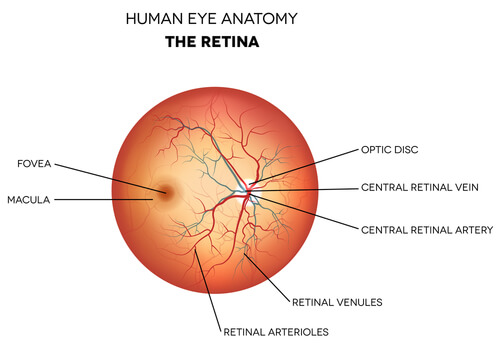
\includegraphics[width=0.5\textwidth]{figures/the_retina.jpg}
\caption{The structure and components of a human retina, refer to
https://www.visioncareofmaine.com/retina-bangor/}
\end{figure}

\subsection{眼底疾病的介绍}
There are several diseases that manifest as retinal impairments, including DR, AMD (age related macular degeneration), Cardiovascular diseases, Glaucoma and so on \cite{badar2020application}. In this paper, we mainly focus on improving the deep learning methods for DR diagnosis. DR is a disease serving as one of the prevalent consequences of diabetes mellitus (DM), caused by fluctuating level of glycemia. When DR is severe, it will become microaneurysms, neovascularization, hemorrhages, cotton wool spots, and exudates in the retinal region. From Figure 2, we can see four zoomed picture of lesions. The first one, the sac-like structure \cite{badar2020application}, enclosed by the yellow box is called microaneurysms, which refers to unusual dilation of retinal capillaries caused by lack of oxygen supply \cite{badar2020application}. The emanation of fluffy white pitches \cite{badar2020application} enclosed by blue box is called soft exudates or cotton wool spots. The lesion enclosed by the black box is called hemorrhages, which refers to the burst of vessels \cite{badar2020application} caused by the blockade in arterioles. The part enclosed by the green box is called hard exudates, which refers to a lesion caused by leakage of fat, proteins and water from walls of retinal vessels \cite{badar2020application}. 
\begin{figure}[h]
\centering
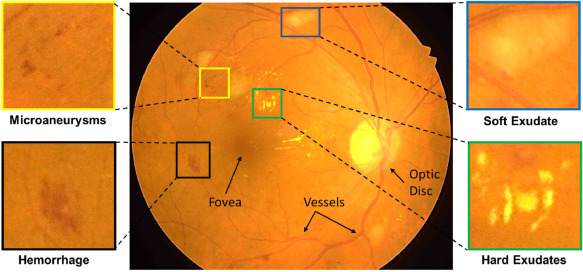
\includegraphics[width=0.5\textwidth]{figures/retinal_image1.jpeg}
\caption{Example of a retinal disease image}
\end{figure}

眼底疾病有哪些,每种眼底疾病的形成原因,以及在眼底图像中的表现(病灶)

\section{基于深度学习的眼底图像分类方法}

该部分内容,主要阐述基于深度学习的眼底图像分类方法的相关知识

\subsection{深度学习方法的原理}

Deep learning is a subfield of machine learning, and they both employ neural network. In a maiden machine learning, we use a simple neural network, including an input layer, a hidden layer and an output layer, to train the machine. Data in a neural network is transmitted from one neural to another one, and this kind of non-deep machine learning requires manual data representation in the form of the features \cite{badar2020application}. This means if we were to use a maiden machine learning, then we need to "teach" the machine about the features of all possible lesions which lead to DR detection. A deep learning machine, with its ability to conduct hierarchical feature extraction \cite{badar2020application}, has self-learning ability and does not require handcrafted features to be fed.
通过阐述深度学习方法的原理,说明深度学习方法与非深度学习方法(比如:神经网络)有着很大的不同,从而说明在理论上,深度学习方法是一种眼底疾病诊断的有效方法。

\subsection{深度学习中的特征提取方法}
In deep learning, particularly in retinal image analysis, a CNN (convolutional neural network) is usually used to better extract the features of the input image. A convolution operation uses dozens of random filters to "slide" across the input image, and creates the same number of filtered images called feature map, and passes them to the processing layers like maxpooling or dropout. The convolution operation repeats for several times, and eventually forms a very deep neural network. By performing multiple convolution operations, CNN's performance can 
surpass a simple neural network. With the power of CNN, a deep learning model can extract high level features from the images, and thus detect the DR more accurately.
阐述卷积算子提取眼底图像特征的原理、以及深度学习方法中核心的问题,即能够提取眼底图像的高级特征,从而能够比其他方法,更准确地诊断眼底疾病。

\subsection{训练数据对深度学习的重要性}
Researches have indicated that, the increase of data imbalance will have negative effect on the performance of classification models \cite{mazurowski2008training}. In the experiment mentioned above \cite{mazurowski2008training}, the data with different class prevalence indexes were fed into the same group of neural network models, and the result shows that as the class prevalence index gets closer to 0.5, which represents a balanced class prevalence, the performance of the model increases, and eventually leads to the conclusion about the impact of imbalance dataset on the performance of neural network models. 
Moreover, researches have also shown that increasing the size of dataset can lead to better accuracy and improved generalization capability \cite{ajiboye2015evaluating}. In another experiment \cite{ajiboye2015evaluating}, three datasets with the size of 400, 800, 1200 were fed into the same training model with the same data partition ratio. The result show that the error of the models to process unknown data decreases as the size of the dataset increases, which lead to the conclusion of the impact of dataset size referred above. Therefore, by analysing these two experiments conducted, we can learn that it is very beneficial to create a balanced dataset with a considerable size if we want to achieve any satisfying performance.
通过引述相关论文,阐述训练数据数量和类别数据的均衡对模型训练的重要性。

\section{本文提出的诊断眼底疾病的深度学习方法}

这部分主要介绍本文使用的深度学习网络结构、以及数据增强方法

\subsection{网络结构}

We use four models \cite{model1}\cite{model2}\cite{model3}\cite{chollet2016building} with different complexities to verify our hypothesis about the impact of balancing the dataset and expanding the size of the dataset. The model that we focus on most is the model 1 \cite{model1}, which is described as a mimic of the VGG16 neural network but with a smaller size. The model 1 contains five main structures: the first one is the input module, the second and third are convolution modules, the fourth is a flattening module, and the last one is the softmax output module. The first module contains a Con2D layer, a "relu" activation layer, a batch normalization layer, a Maxpooling layer and a dropout layer. The second and third module both have two groups of Con2D, "relu" activation, batch normalization, then a maxpooling and a dropout. The fourth module has a flattening layer, a dense layer, a "relu" activation layer, a batch normalization layer and a dropout layer. The last module has a dense layer and a "softmax" activation layer. For other three models, they all have a simpler structure than the model 1, and use simple layers, including Con2D, "relu" activation, maxpooling and dropout layers.

介绍本文的网络结构,阐述其中关键的计算,例如:卷积核提取特征、pooling数据降维避免过拟合、及其他

\subsection{数据增强方法}
In an effort to expand and balance our dataset, we employ several augmentation methods to produce augmented images for the purpose of training. These augmentation methods include rotation, width and height shifting, rescaling, zooming, horizontally and vertically flipping, brightness and filling. We compare with two pairs of original and augmented images, from Figure 3 to Figure 6.  

介绍本文用到了哪些数据增强方法,以及这些方法对图像做了哪些处理,用处理前后的图片做对比说明。
\begin{figure}[h]
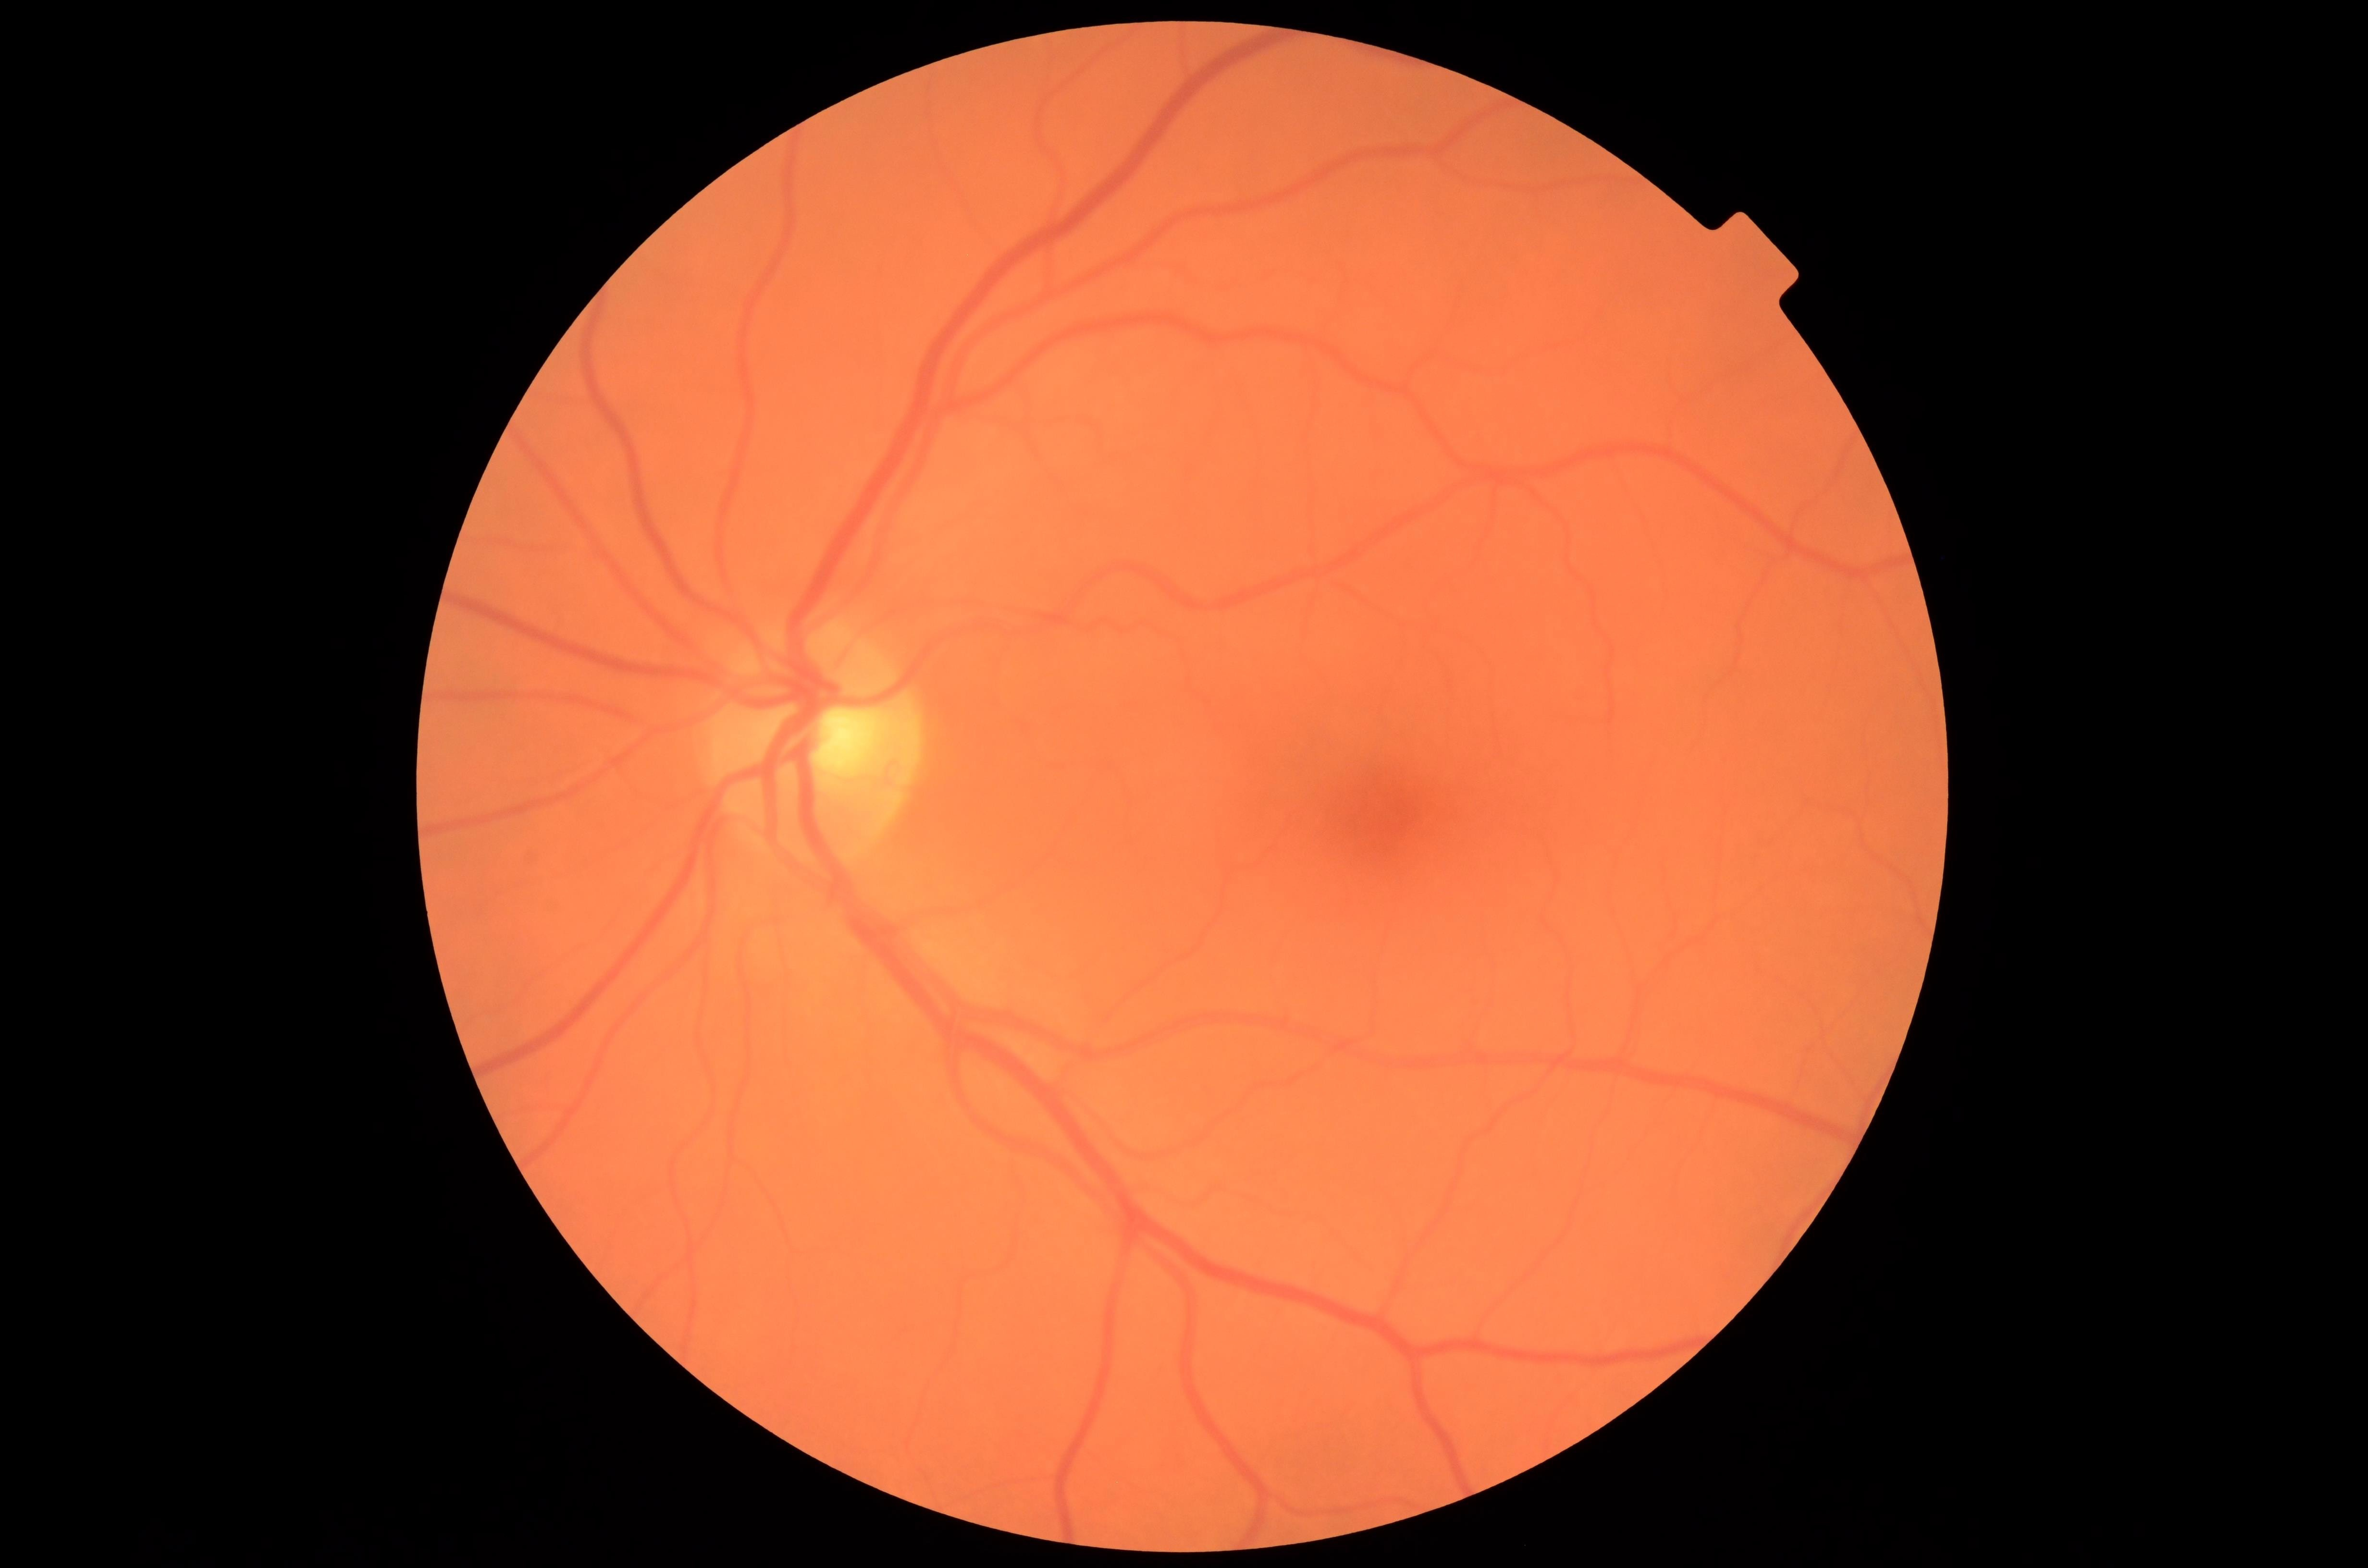
\includegraphics[width=0.5\textwidth]{figures/zero.31_leftN.jpeg}
\caption{Example of an original retinal image (degree 0)}
\end{figure}

\begin{figure}[h]
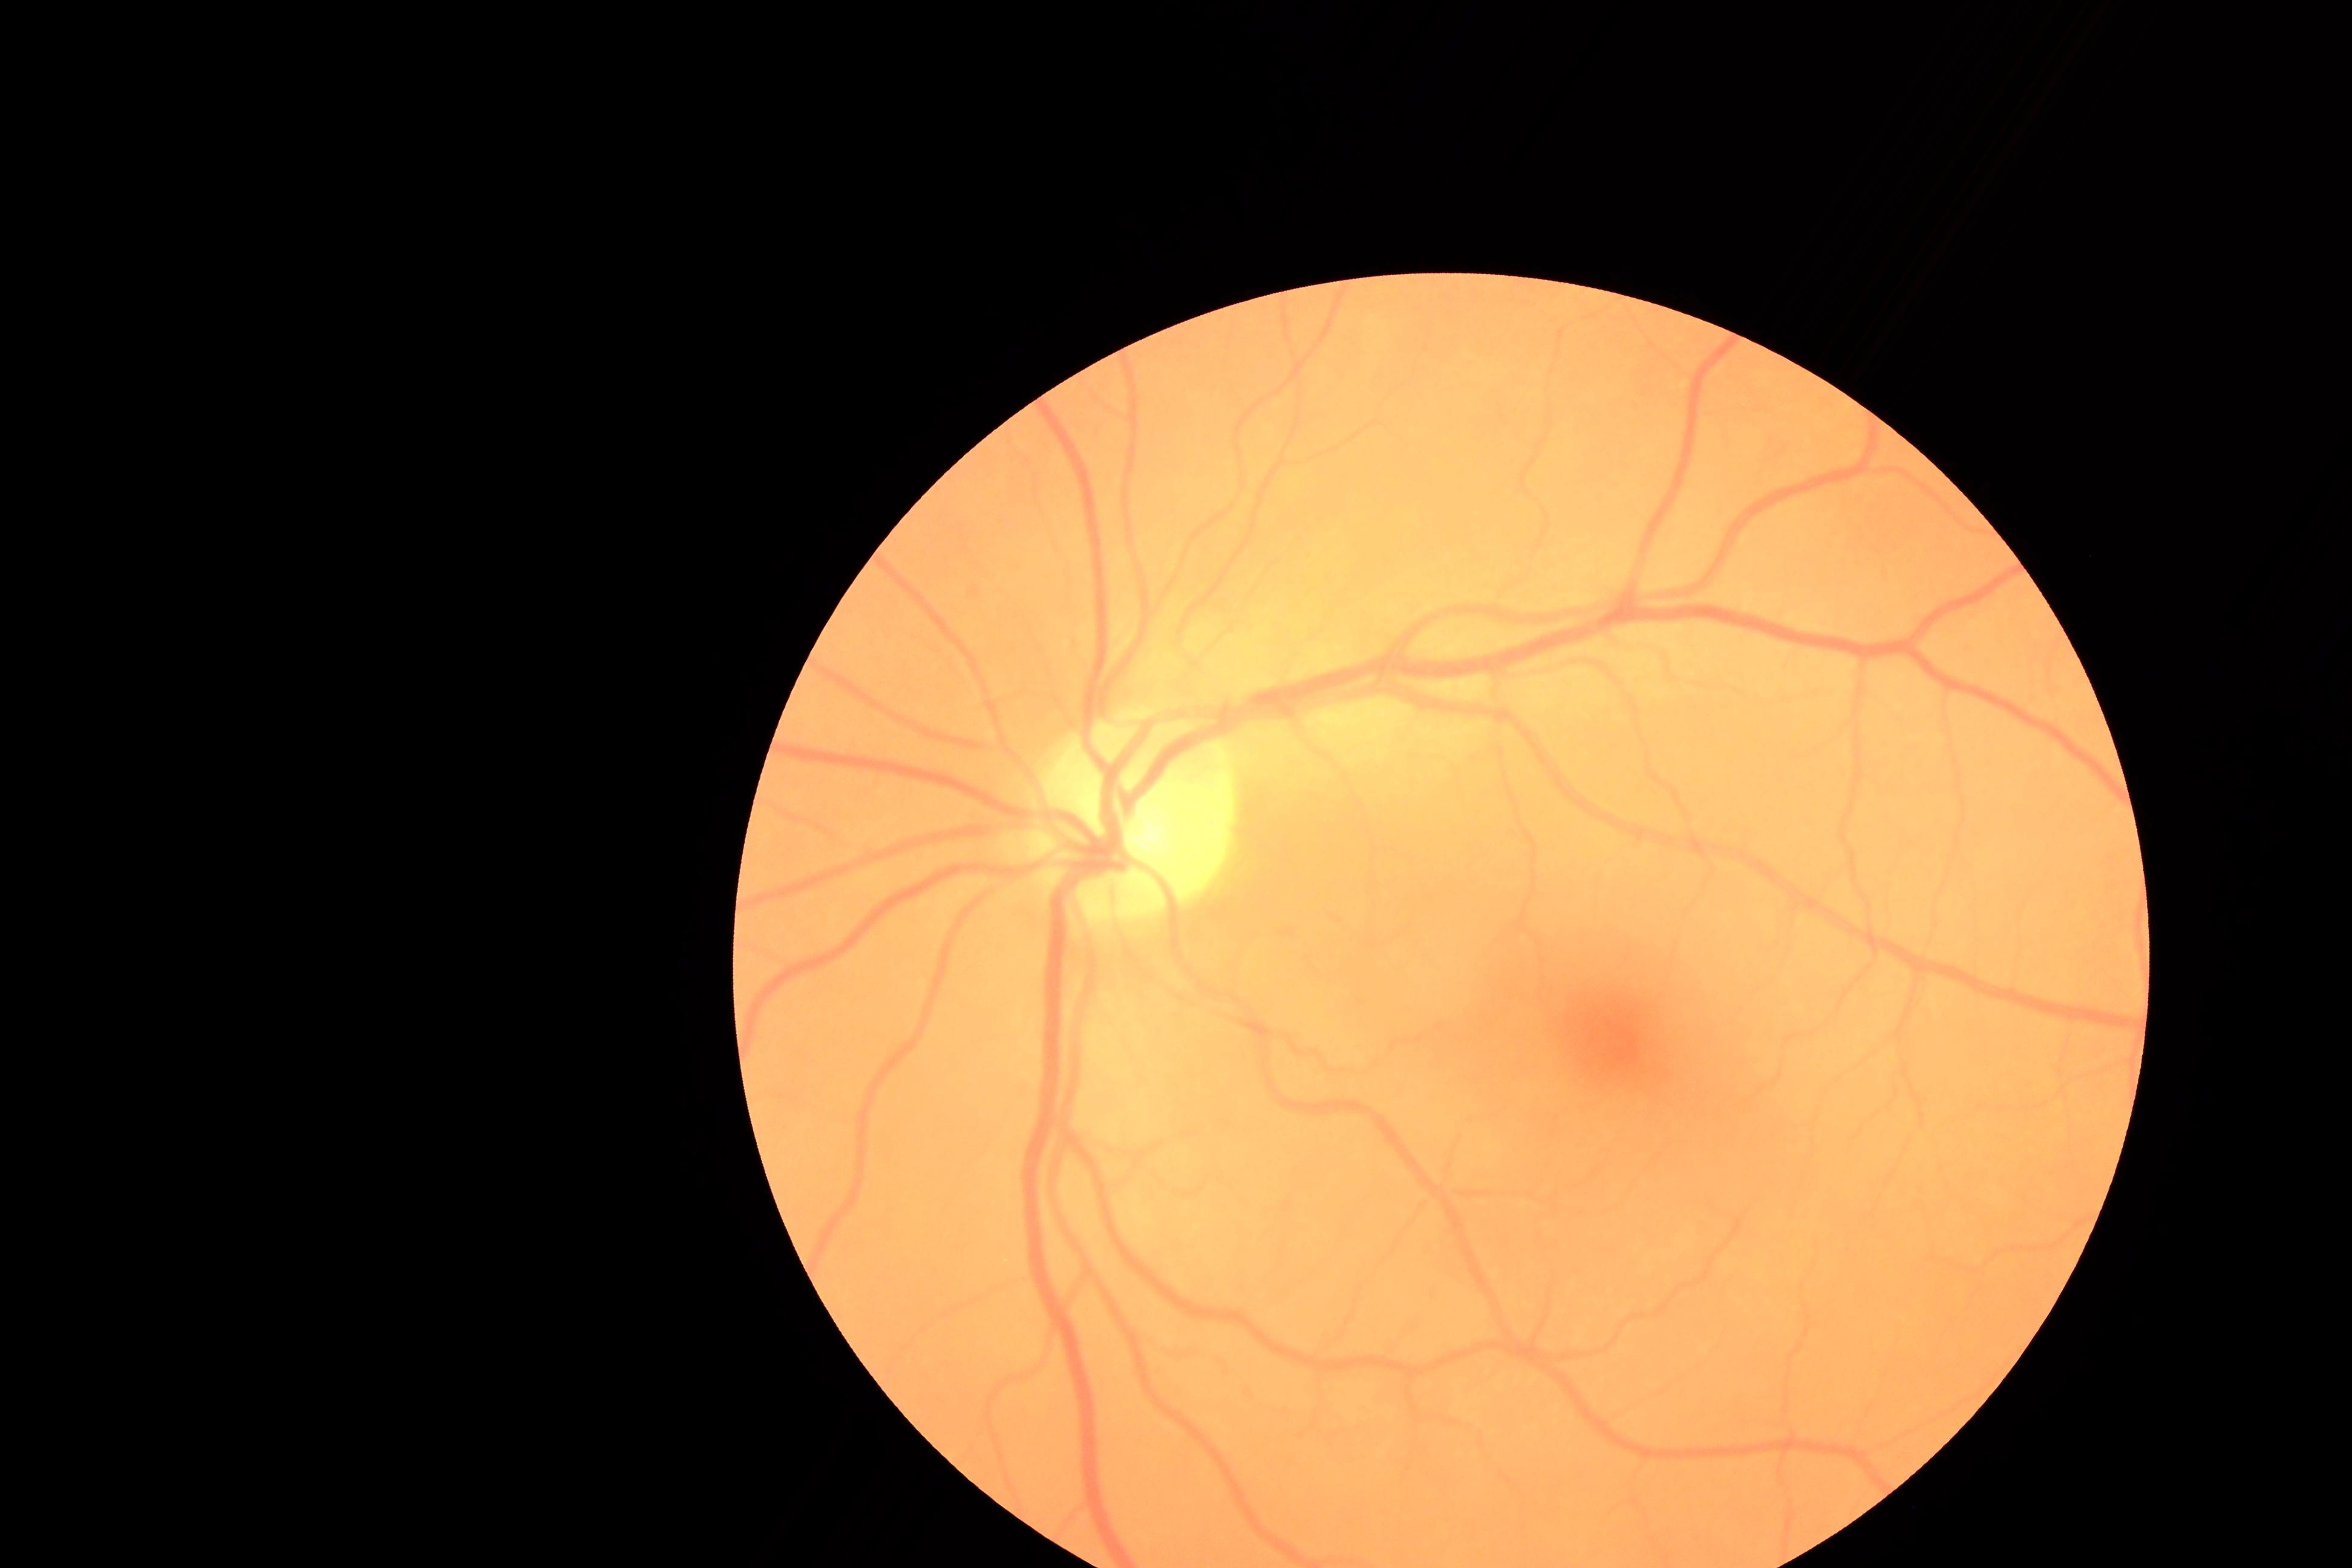
\includegraphics[width=0.5\textwidth]{figures/0._0_261439.jpeg}
\caption{Example of an augmented retinal image (degree 0)}
\end{figure}

\begin{figure}[h]
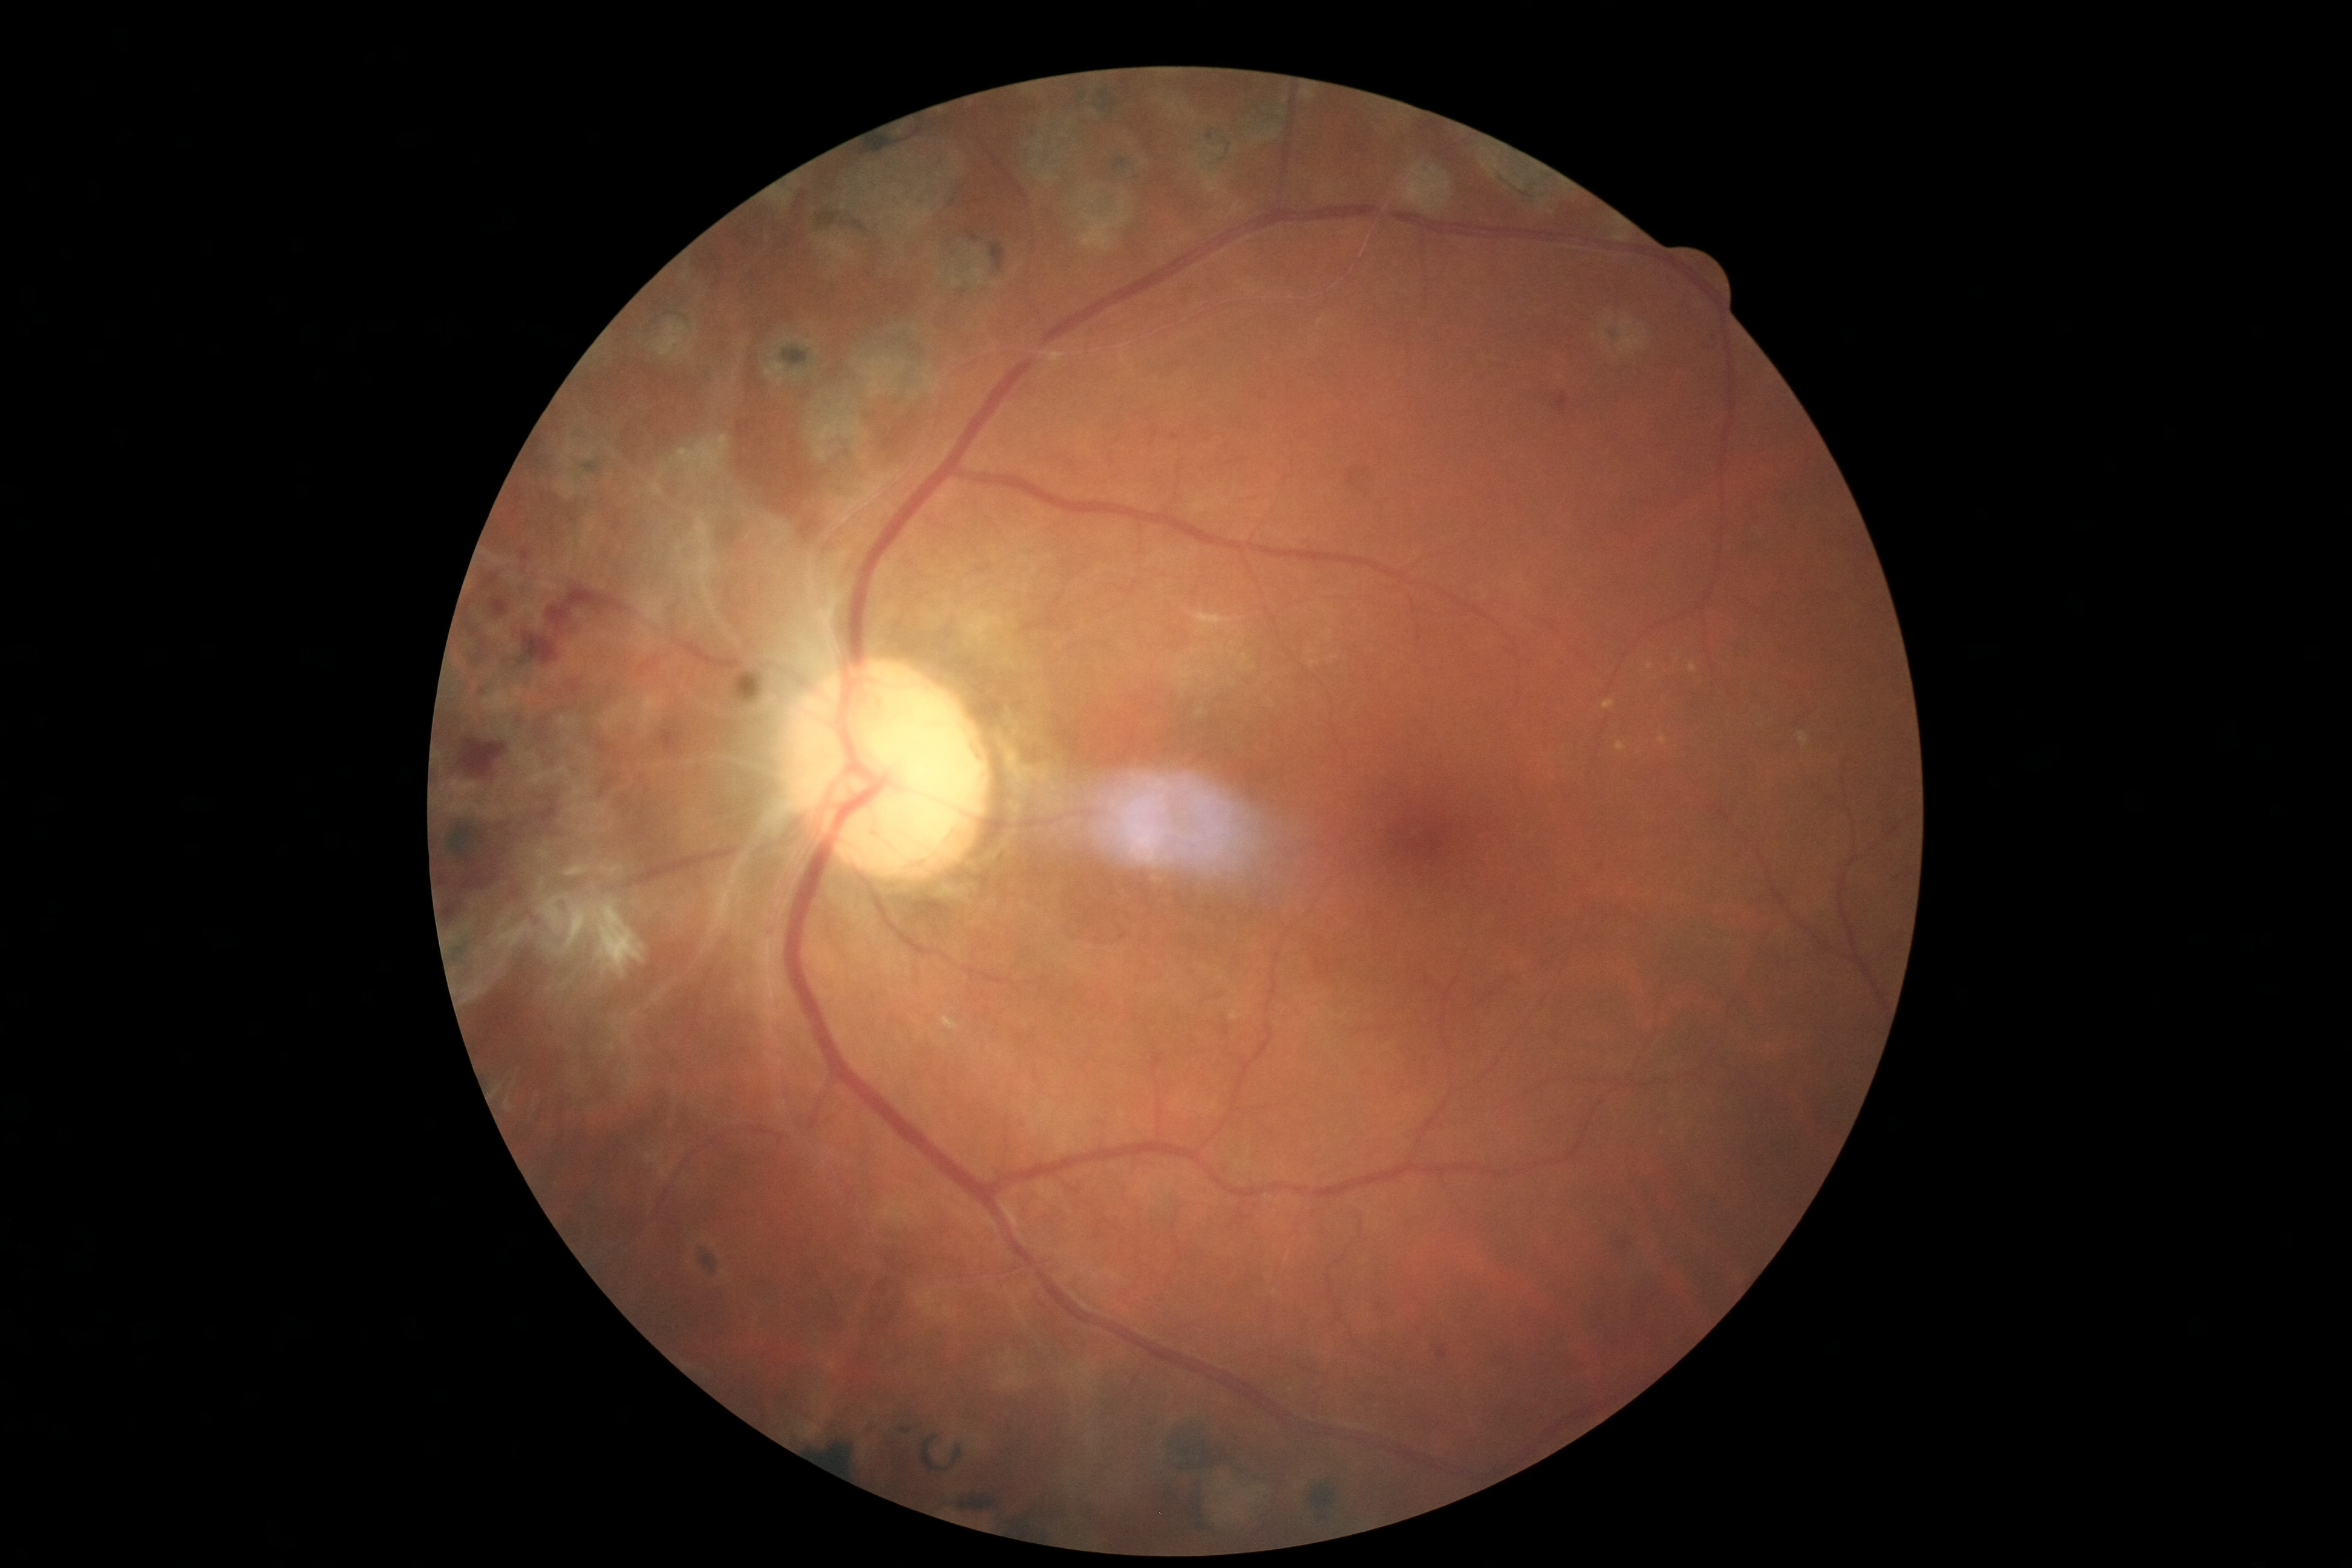
\includegraphics[width=0.5\textwidth]{figures/four.294_leftN.jpeg}
\caption{Example of an original retinal image (degree 4)}
\end{figure}

\begin{figure}[h]
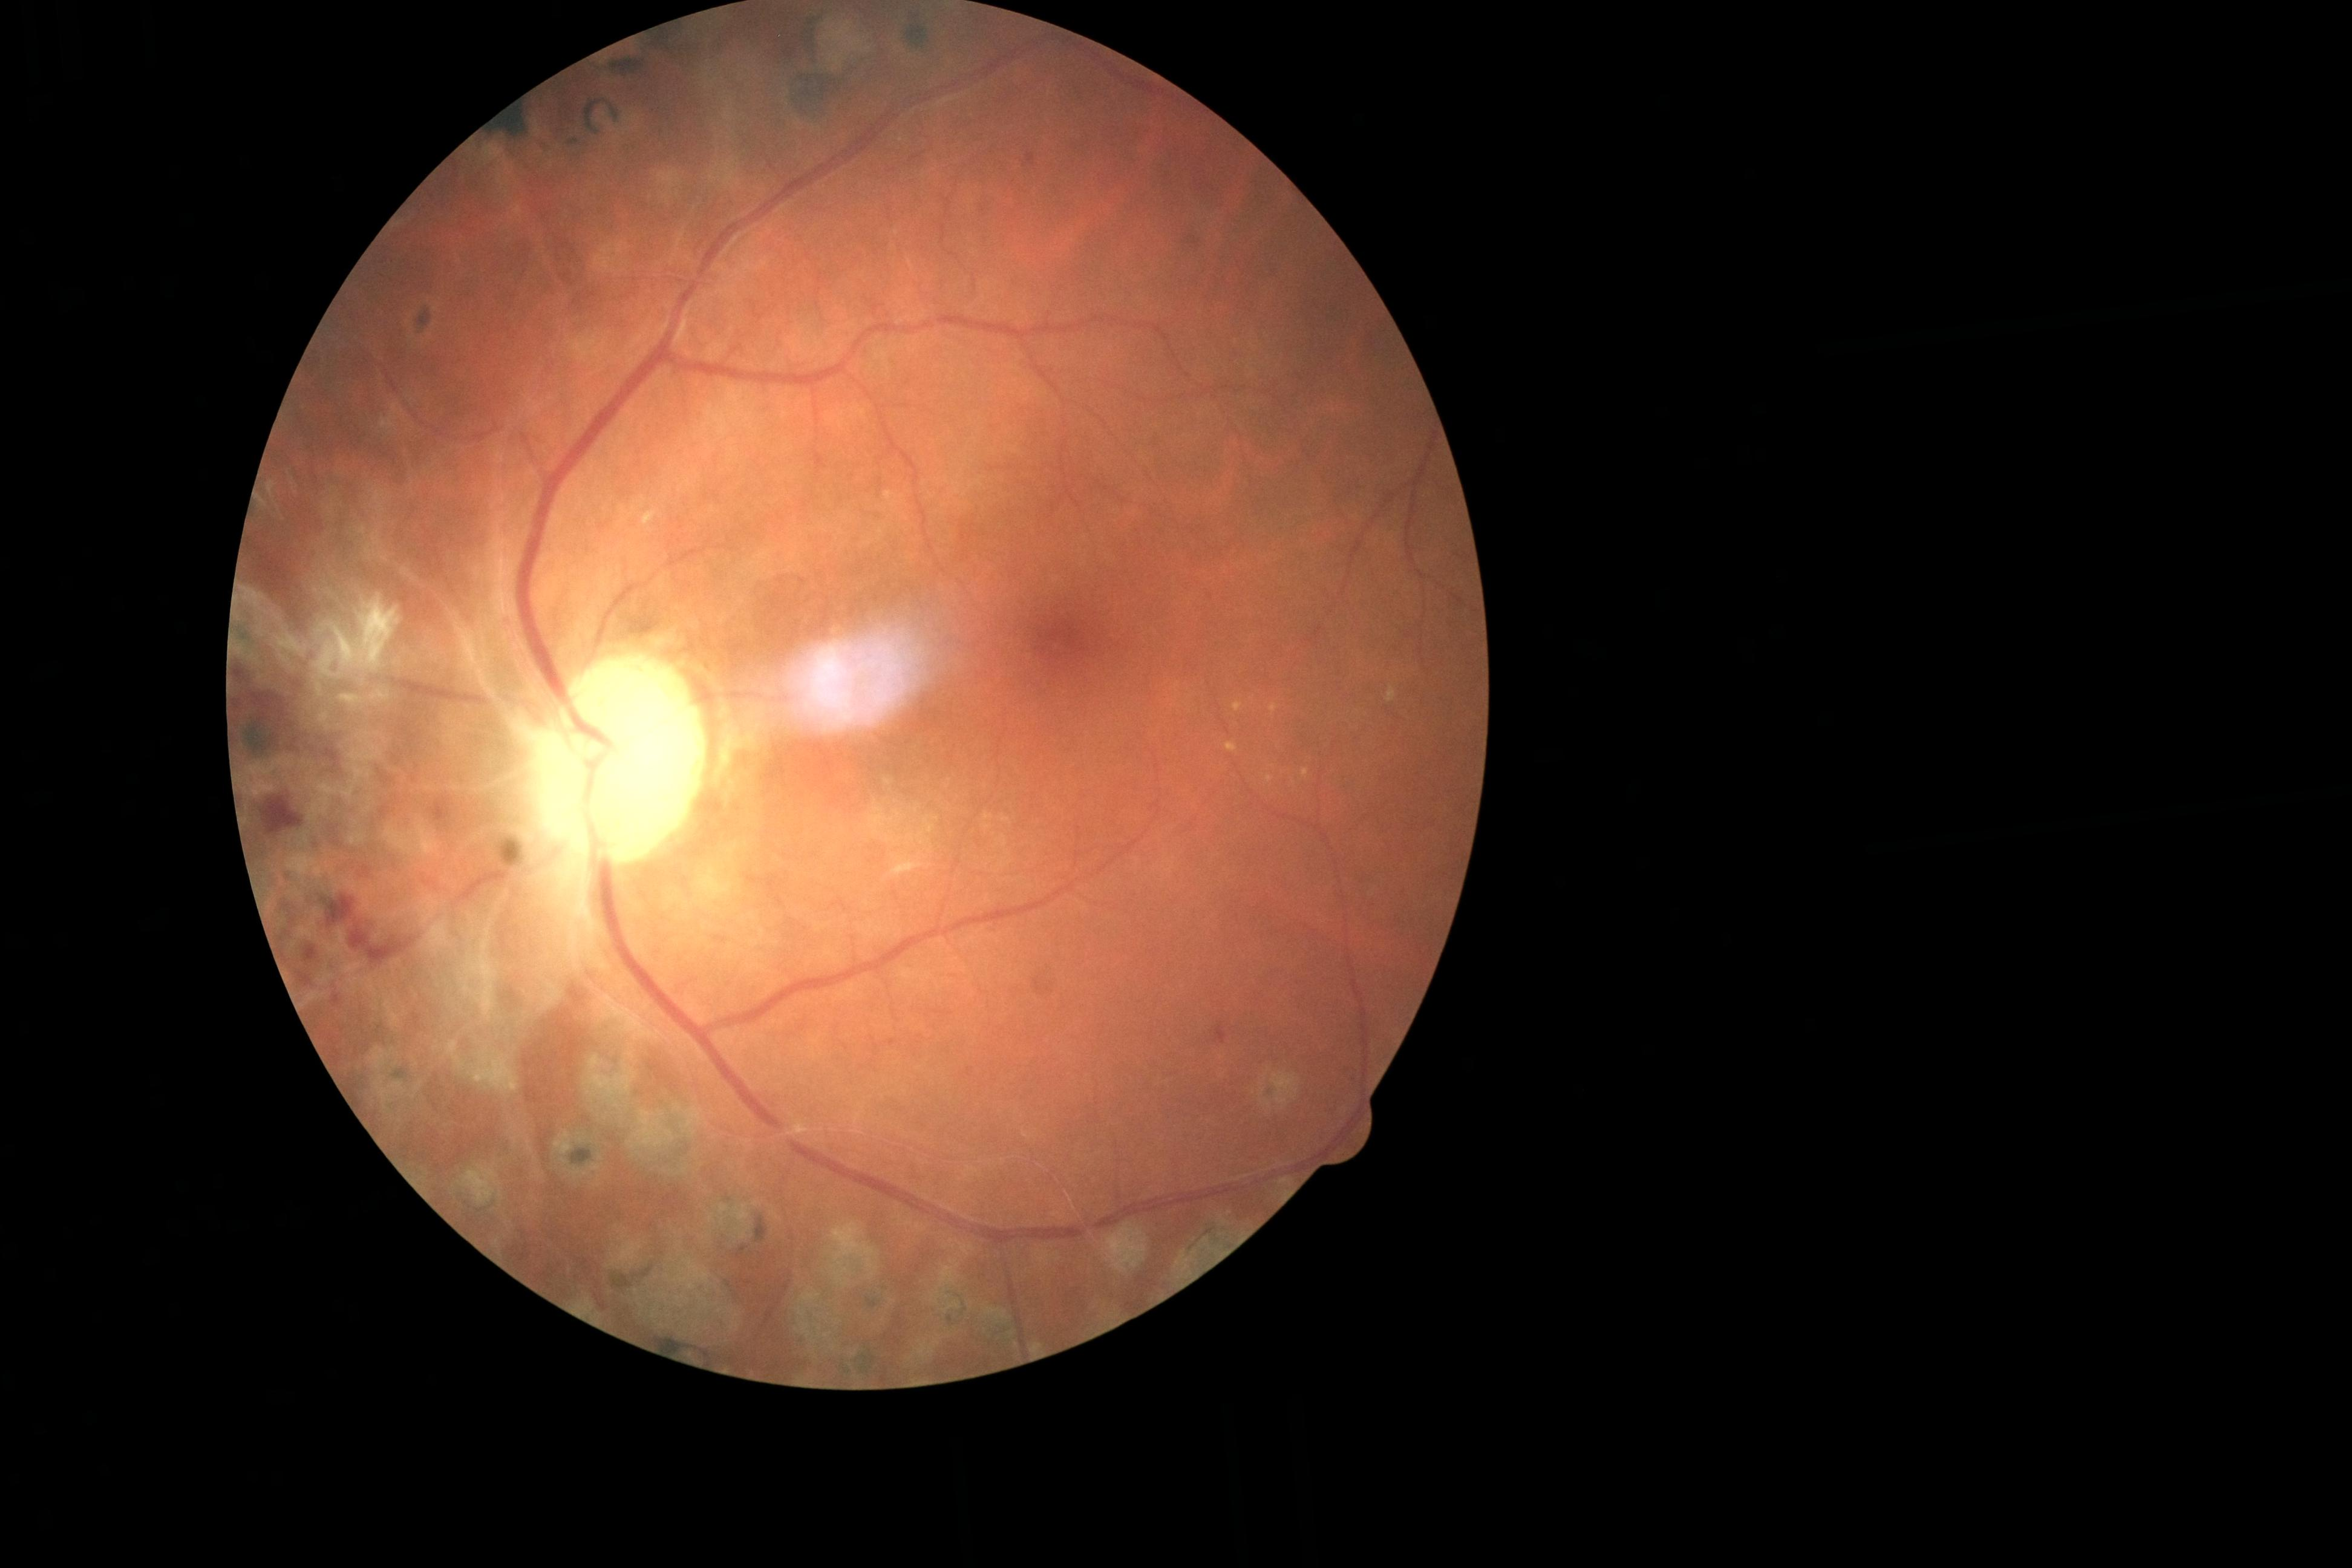
\includegraphics[width=0.5\textwidth]{figures/4._0_1293792.jpeg}
\caption{Example of an augmented retinal image (degree 4)}
\end{figure}


\section{对比实验}
阐述使用的数据增强方法后,同一种网络结构,训练得到的模型,其性能得到了提升。
\subsection{数据集介绍}

本实验所用的数据集原图全部来自于世界上最大的数据科学社区kaggle,https://www.kaggle.com/c/diabetic-retinopathy-detection/data。目前任何人都可以通过浏览以上的网址进行眼底图片的下载。kaggle的眼底图片分为五对数据包,每对分别有训练和测试两个数据包,所以数据标签都存储在了一个csv文件中。本实验主要使用了全部五个训练数据包,我们将所有标签的图片都放在了同一个文件夹中,并将与每个图片对应的标签都加在了它们的文件名中,以便之后的数据处理。

Kaggle眼底图片的标签分为五类,0类为阴性,1类为轻度,2类为中度,3类为重度,4类为糖尿病视网膜病变增殖。由于客观上这些类别发生的纪律性不同,所以每个数据包中的每类所含的图片数量也相差较大。在我们将五个训练数据包合并之后,各个类别的图片的数量为:0类13423张,1类1312张,2类2755张,3类449张,4类384张, 同时这个数据集也是用于训练1号模型的数据集。在我们使用了数据增强后的数据的每个类别的数量:0类13306张(原图), 1类13422张(增强), 2类13244张(增强), 3类13235张(增强), 4类13216张(增强),同时这个数据集也是用来训练2号模型的数据集。

All the data used by this experiment come from Kaggle, which is one of the largest data science communities in the world. To obtain these data, you simply need to visit their website: https://www.kaggle.com/c/diabetic-retinopathy-detection/data and register a free account. The diabetic retinopathy detection dataset in Kaggle has five zip packages for training, five zip packages for testing, and a csv file for storing the ground truth of all ten packages, and we used the five training packages in our experiment. Before beginning to train, we reorganize the file structure of the Kaggle dataset, by checking the csv file, we find out each image's label, write it on its filename, and divide all training and testing images into two separate folders. After that, we convert all of these images into tfrecords. 

First we will briefly introduce the classification of the Kaggle dataset images. The Kaggle dataset images provided were classified into five severity degrees of diabetic retinopathy. Degree 0 corresponds to no DR, degree 1 corresponds to mild, degree 2 corresponds to moderate, degree 3 corresponds to severe, degree 4 corresponds to proliferative DR. Due the objective conditions, such as the actual unbalance distribution of the number of patients in each degree, the Kaggle dataset is also very unbalanced. We 
merge the images from the five training packages, obtain 13423 images for degree 0, 1312 images for degree 1, 2755 images for degree 2, 449 images for degree 3 and 384 images for degree 4, and we use this image dataset to train our model A. After the augmentation process, we get 13422 original images for degree 0, 13092 augmented images for degree 1, 13244 augmented images for degree 2, 13235 augmented images for degree 3, 13216 augmented images for degree 4, and this image dataset is used to train model B. Note that the degree 0 images are original since there are already sufficient number to make the entire dataset generally balanced. 


介绍采用的数据集来自哪里,数据的情况:数据量、数据类别、每种类别的数据量。
实验中使用了哪几个类别,每个类别用的数据量(数据增强前后的数据量)。

\subsection{实验数据}
\begin{figure}[h]
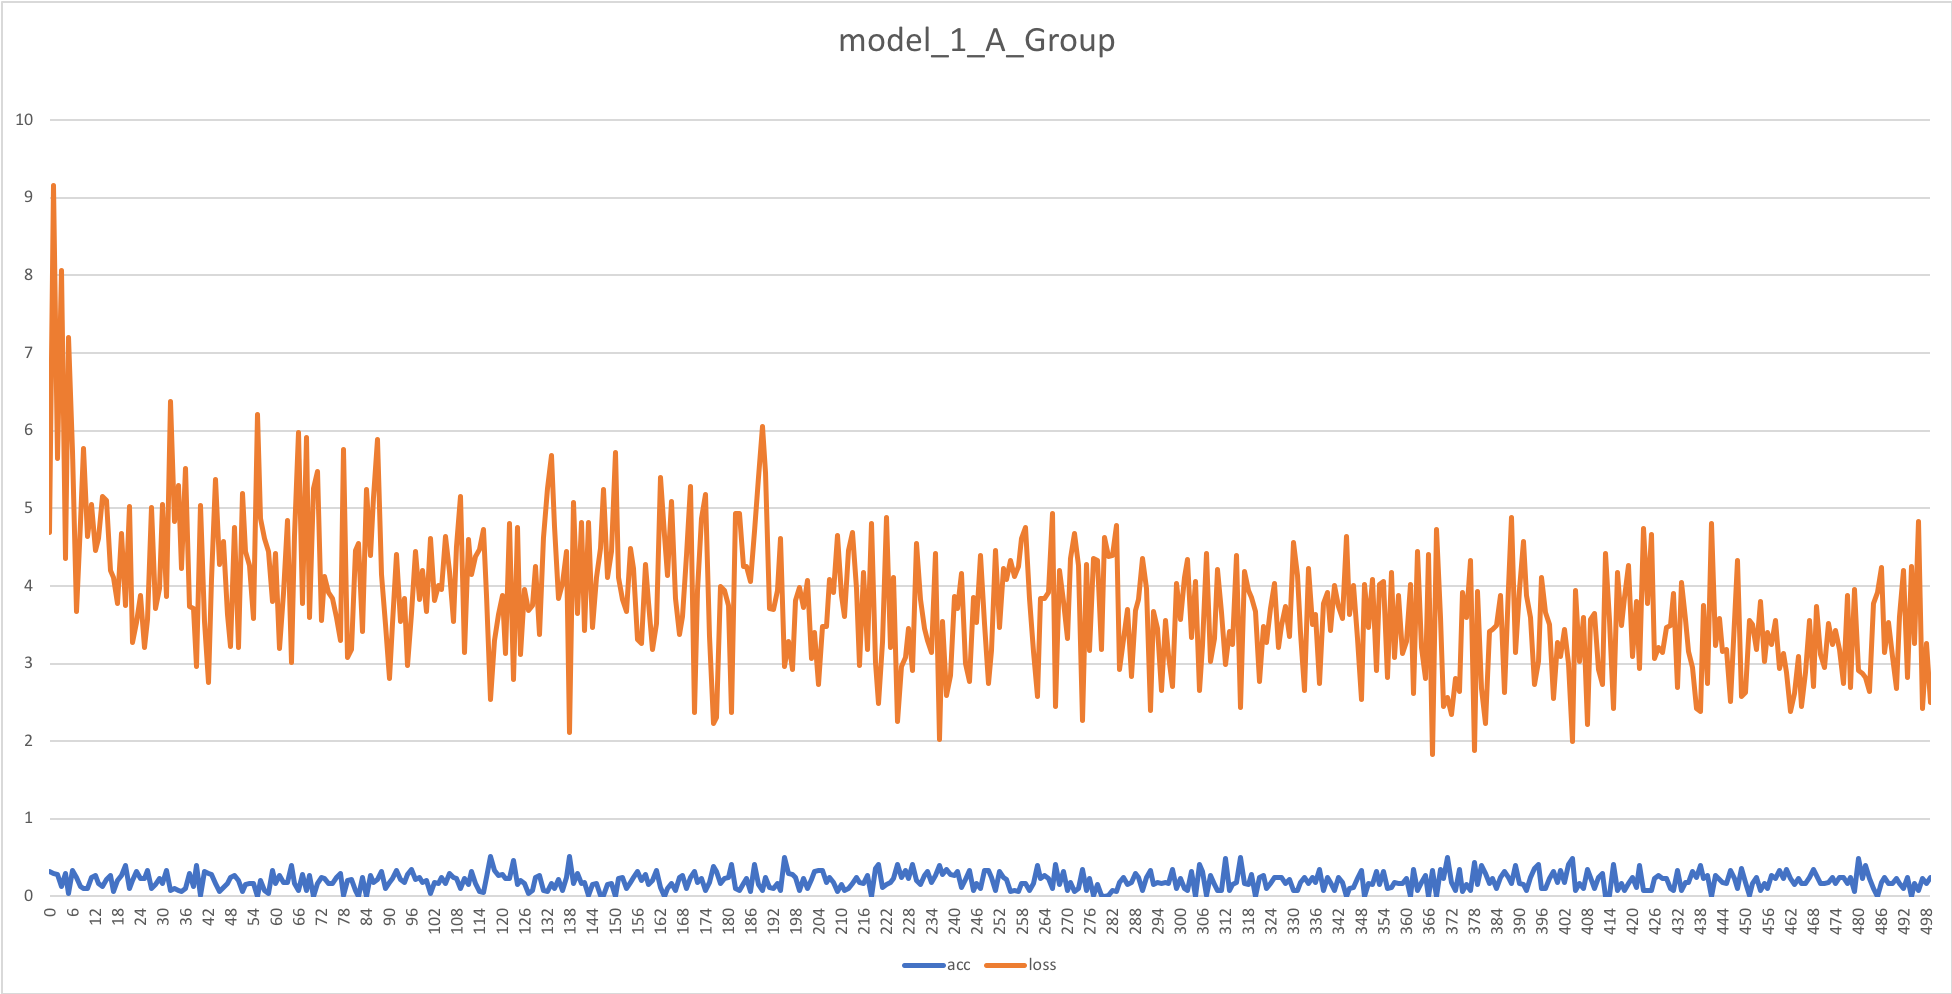
\includegraphics[width=0.5\textwidth]{charts/1A.png}
\caption{Training data of model 1 using original dataset}
\end{figure}


\begin{figure}[h]
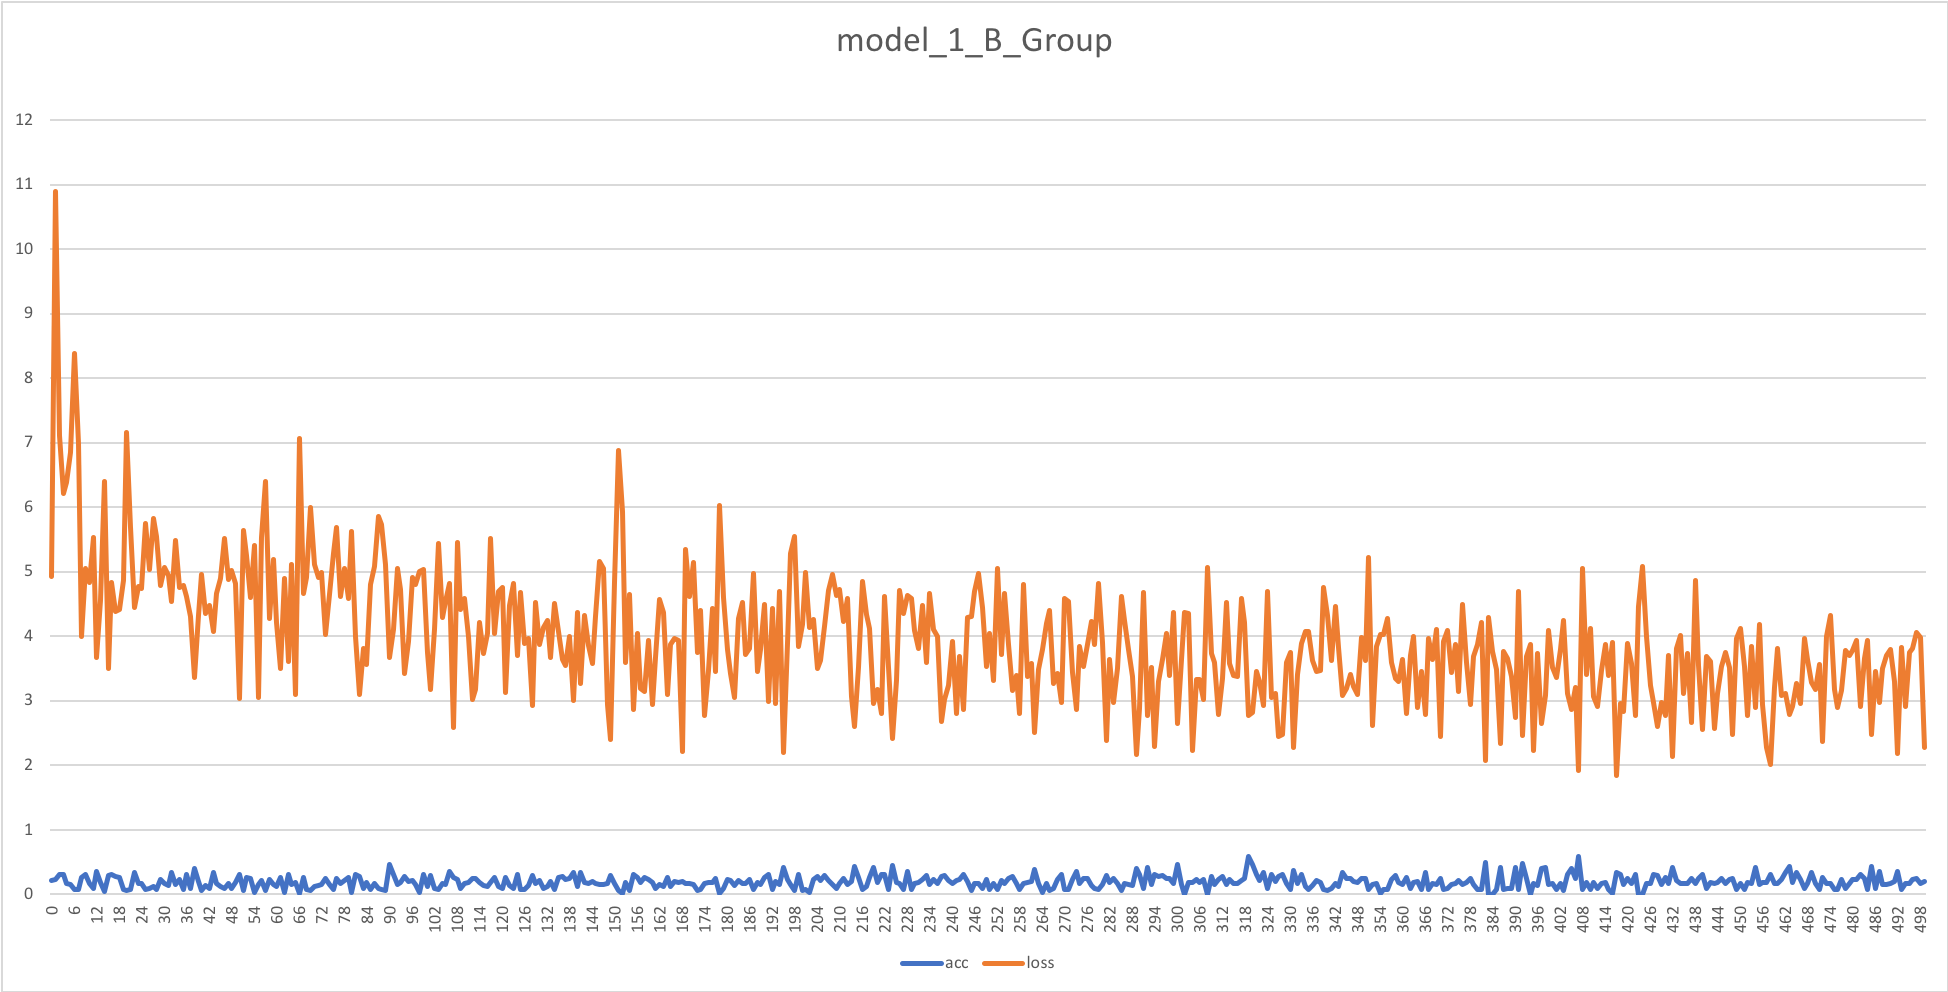
\includegraphics[width=0.5\textwidth]{charts/1B.png}
\caption{Training data of model 1 using augmented dataset}
\end{figure}

\begin{figure}[h]
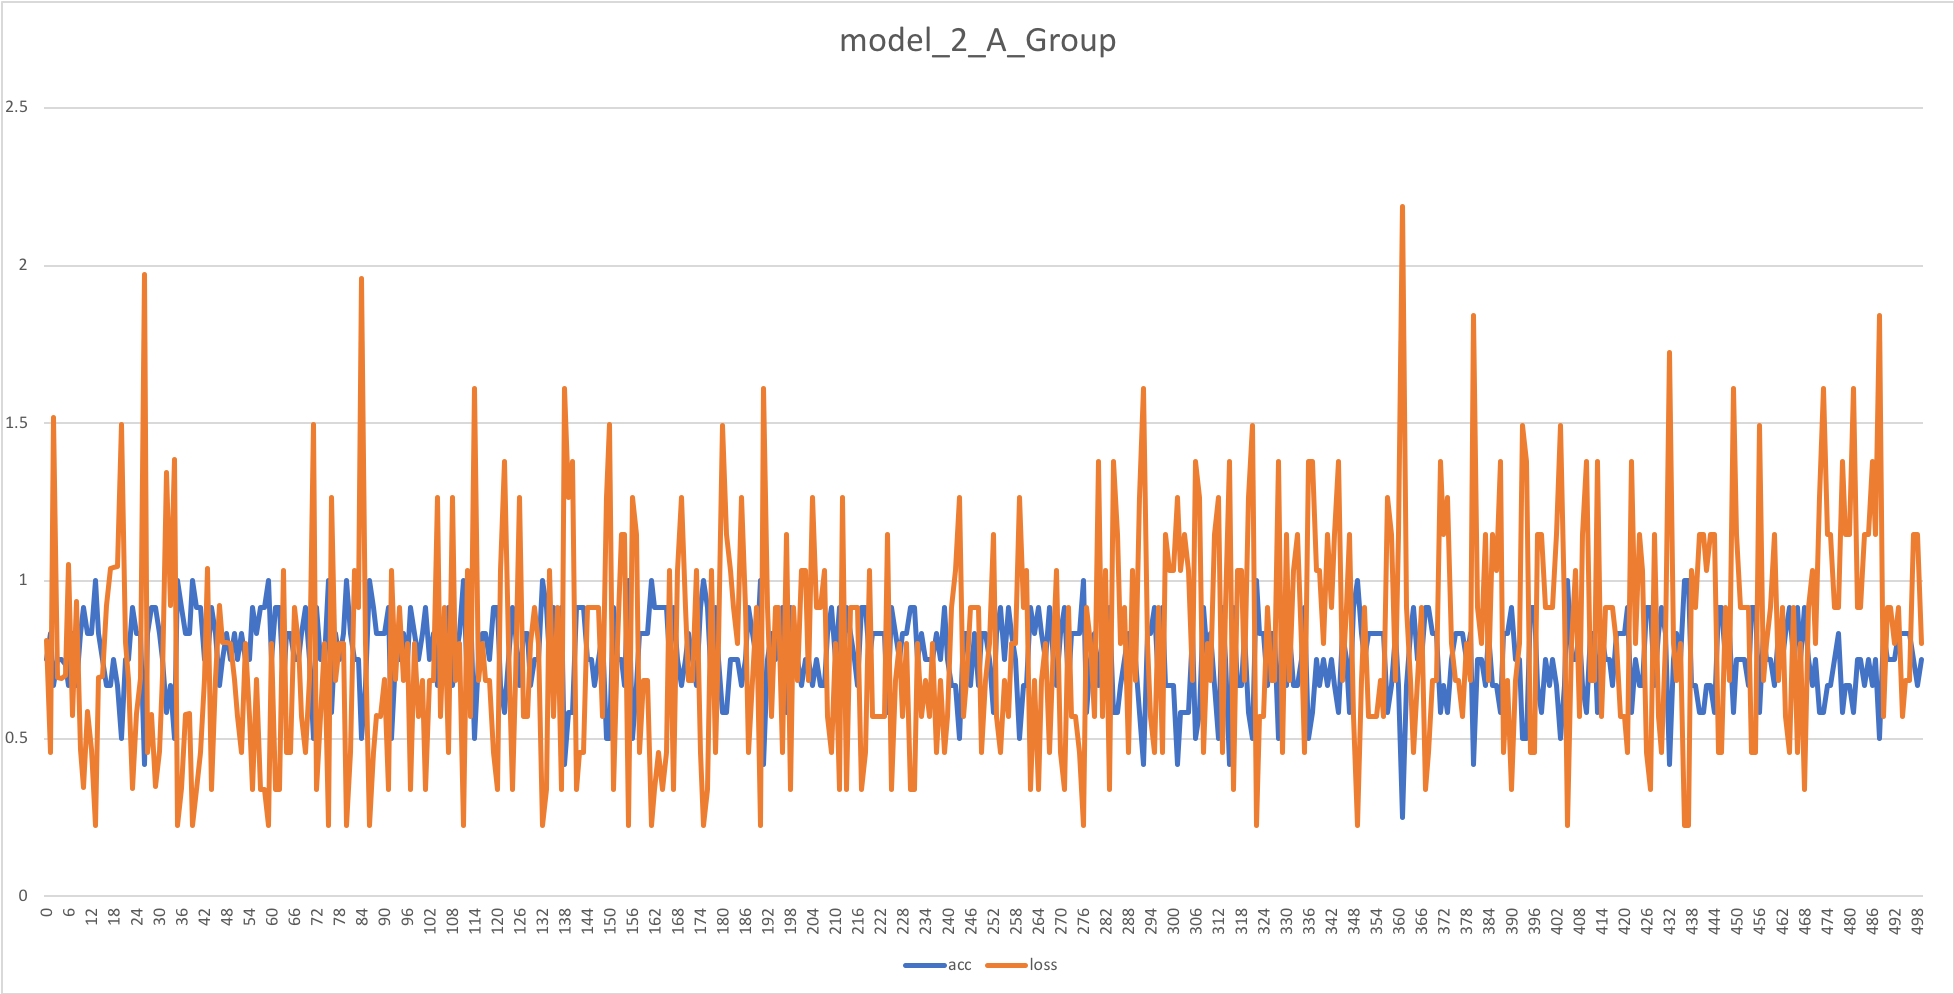
\includegraphics[width=0.5\textwidth]{charts/2A.png}
\caption{Training data of model 2 using original dataset}
\end{figure}


\begin{figure}[h]
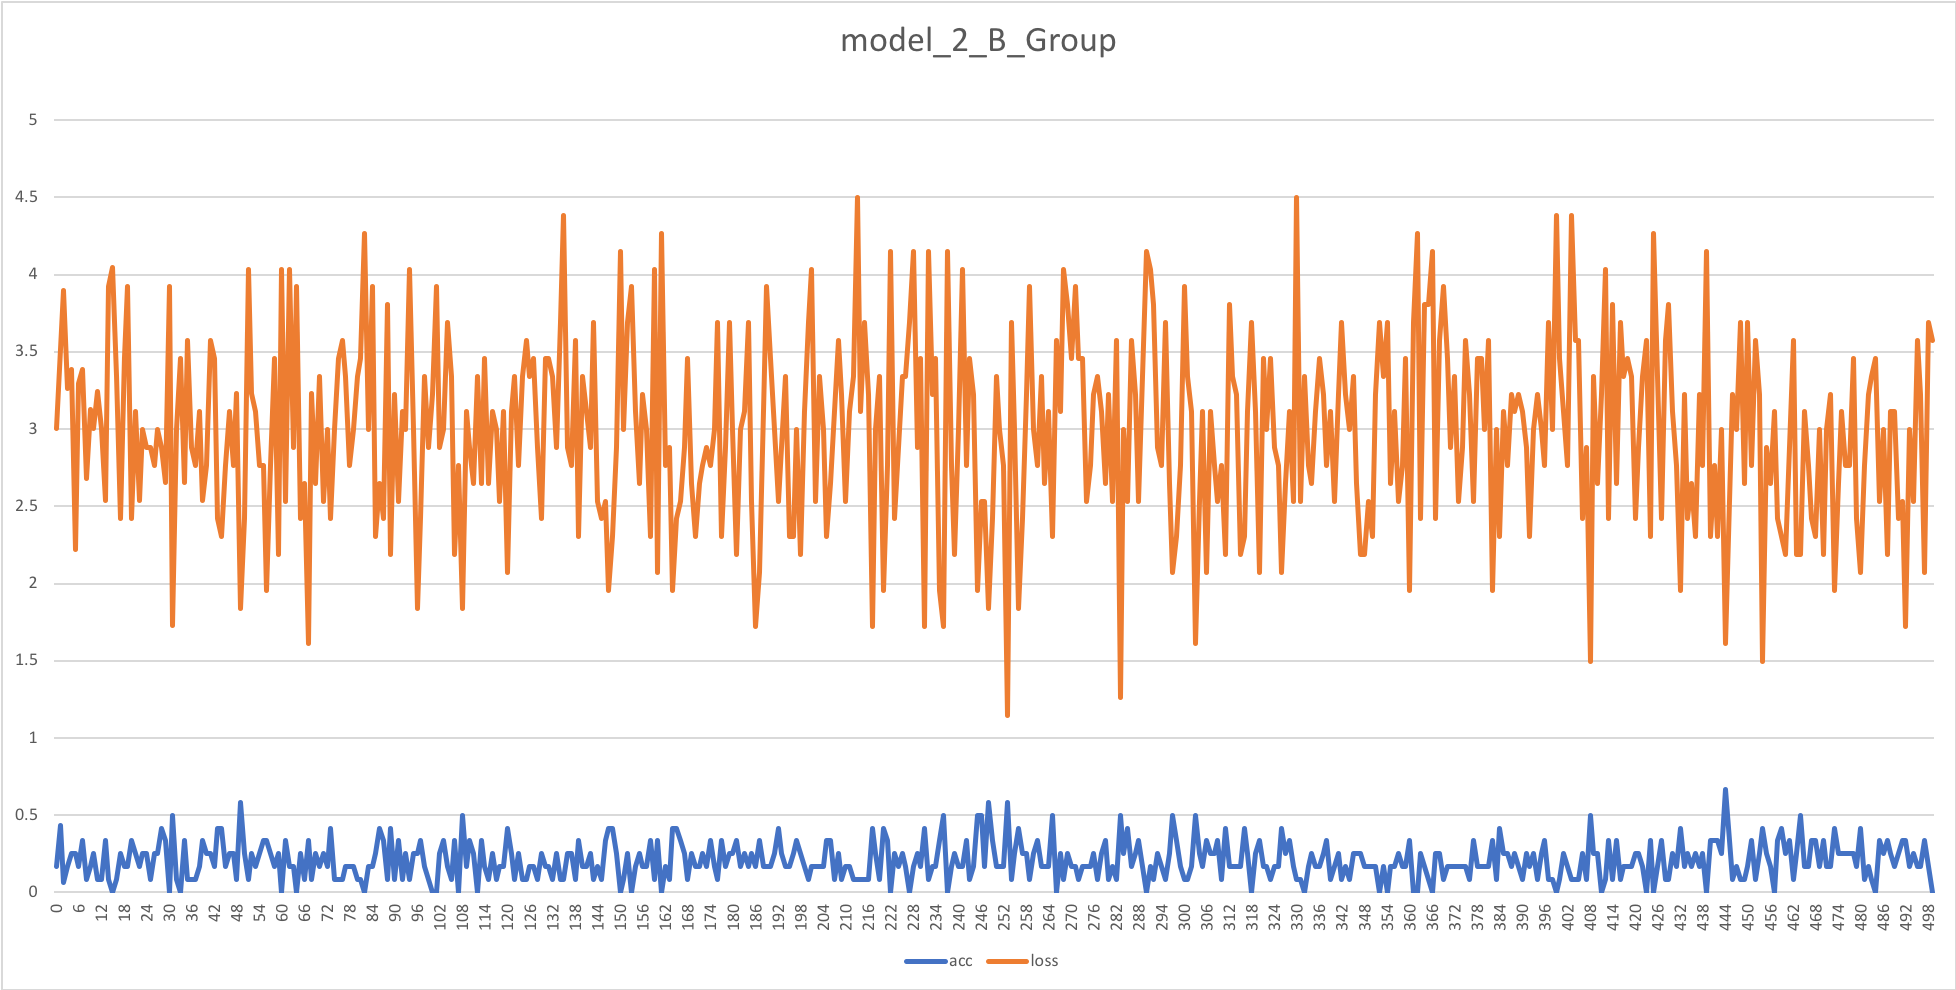
\includegraphics[width=0.5\textwidth]{charts/2B.png}
\caption{Training data of model 2 using augmented dataset}
\end{figure}

\begin{figure}[h]
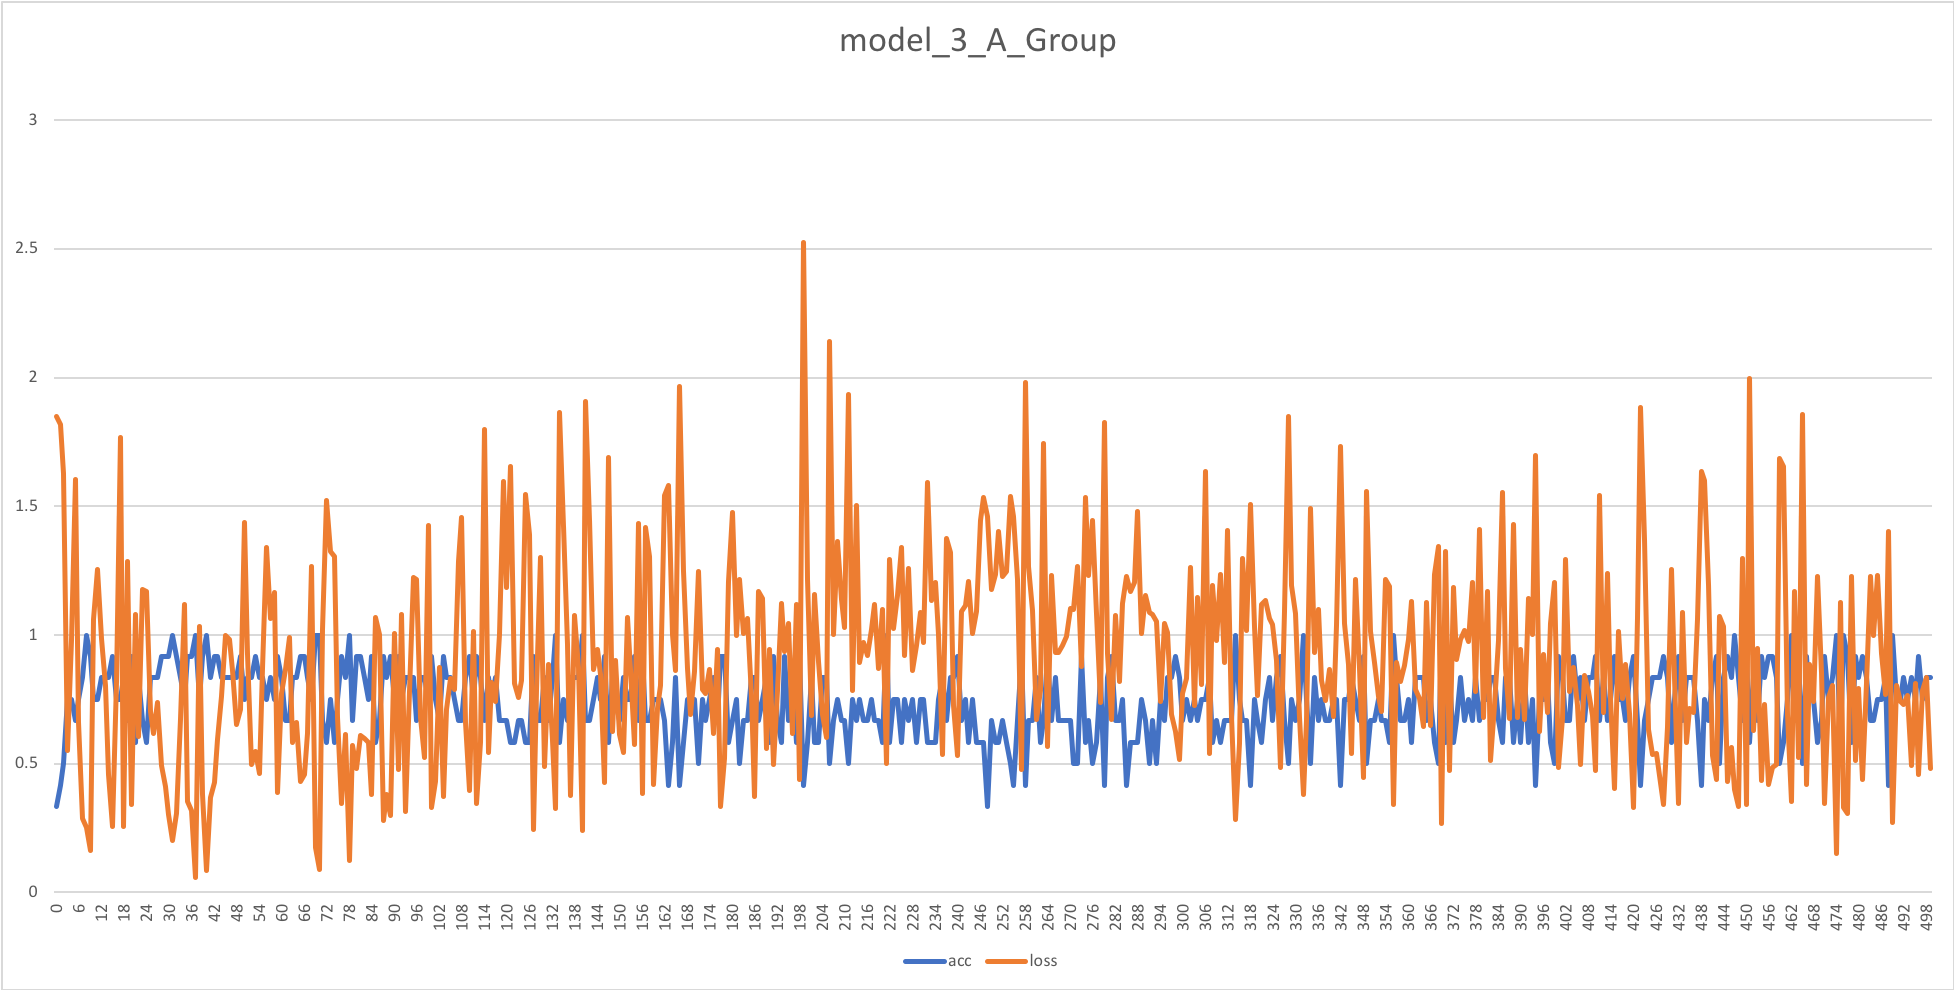
\includegraphics[width=0.5\textwidth]{charts/3A.png}
\caption{Training data of model 3 using original dataset}
\end{figure}


\begin{figure}[h]
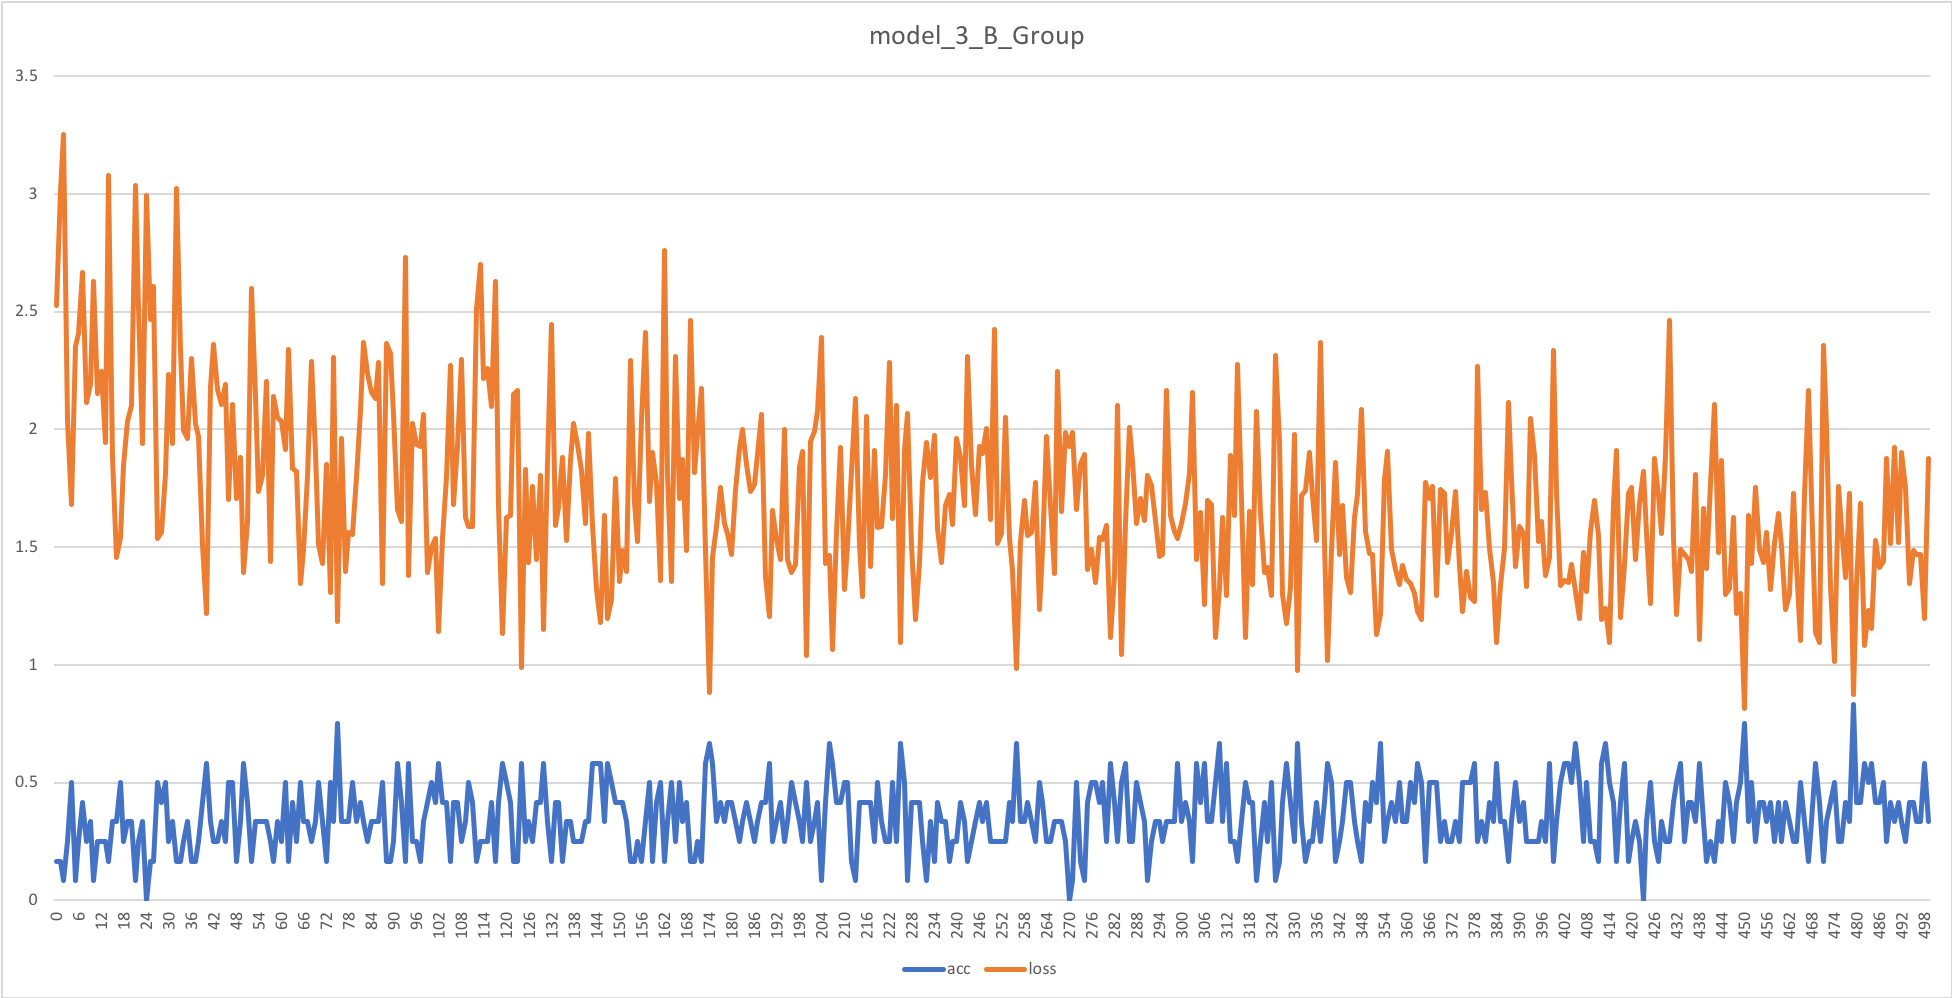
\includegraphics[width=0.5\textwidth]{charts/3B.png}
\caption{Training data of model 3 using augmented dataset}
\end{figure}

\begin{figure}[h]
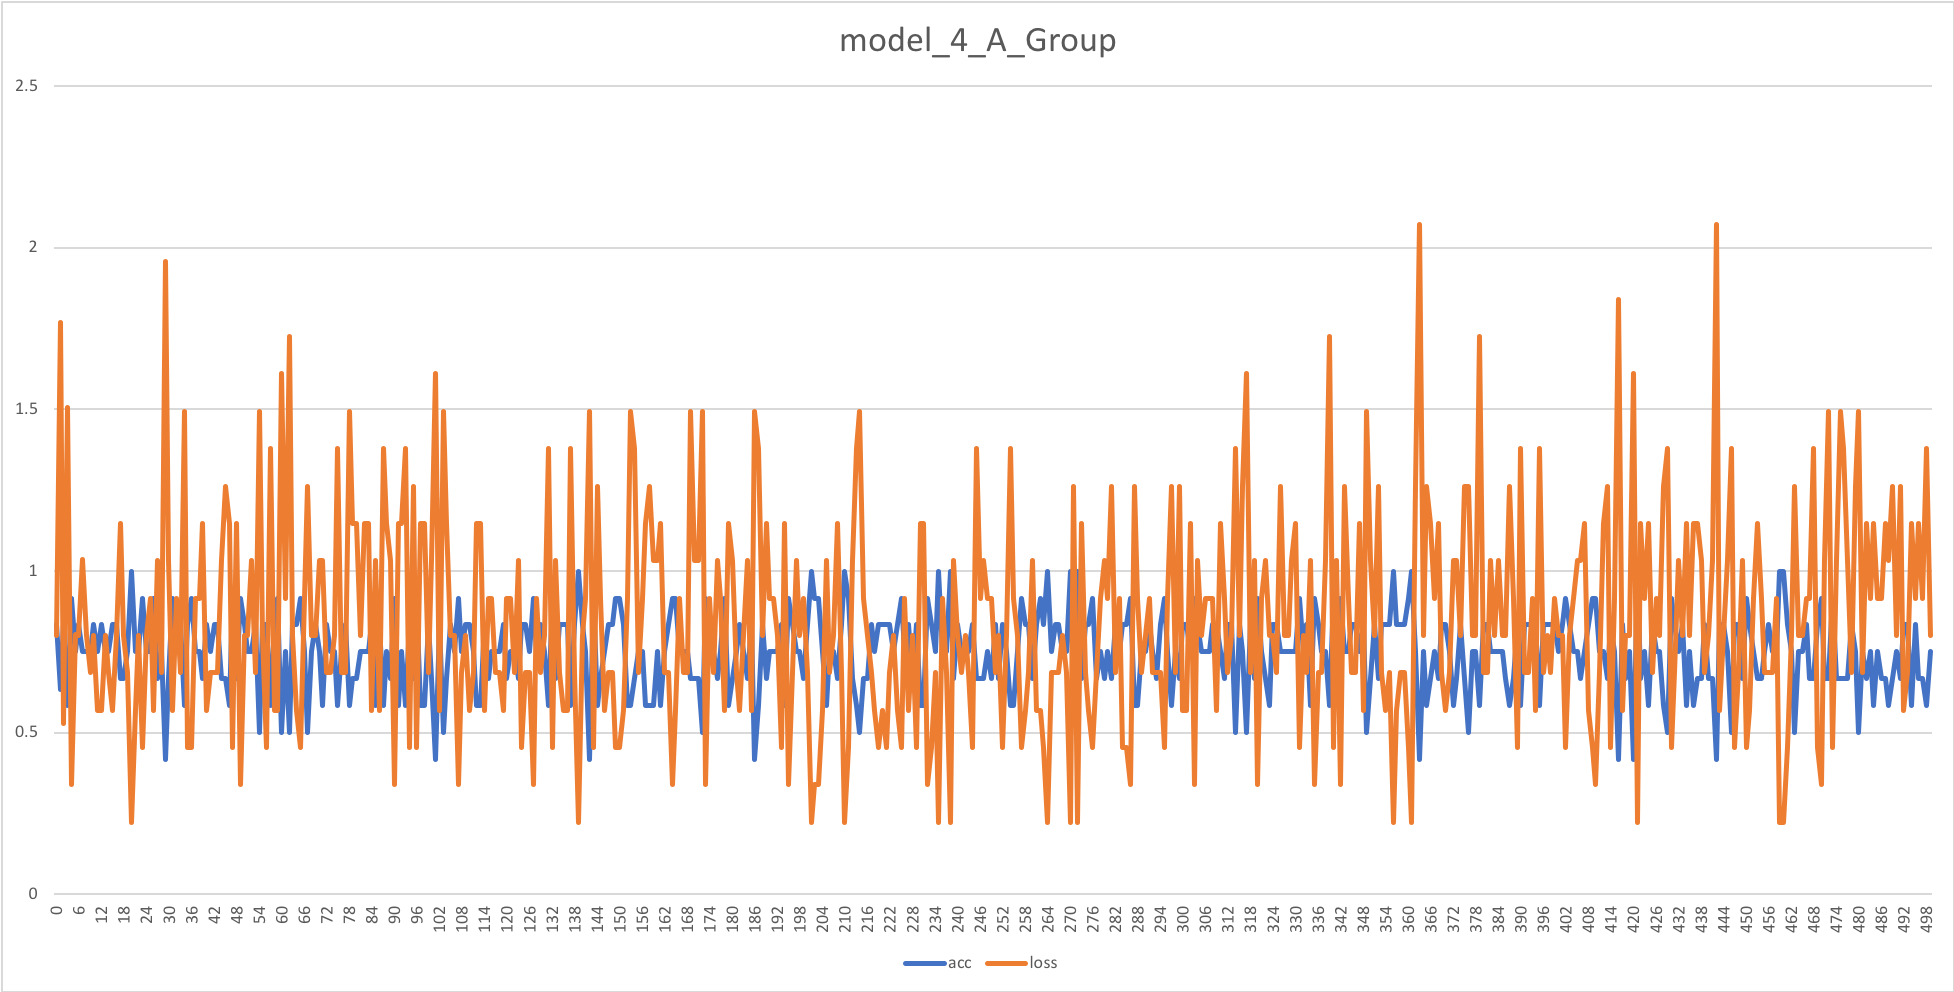
\includegraphics[width=0.5\textwidth]{charts/4A.png}
\caption{Training data of model 4 using original dataset}
\end{figure}


\begin{figure}[h]
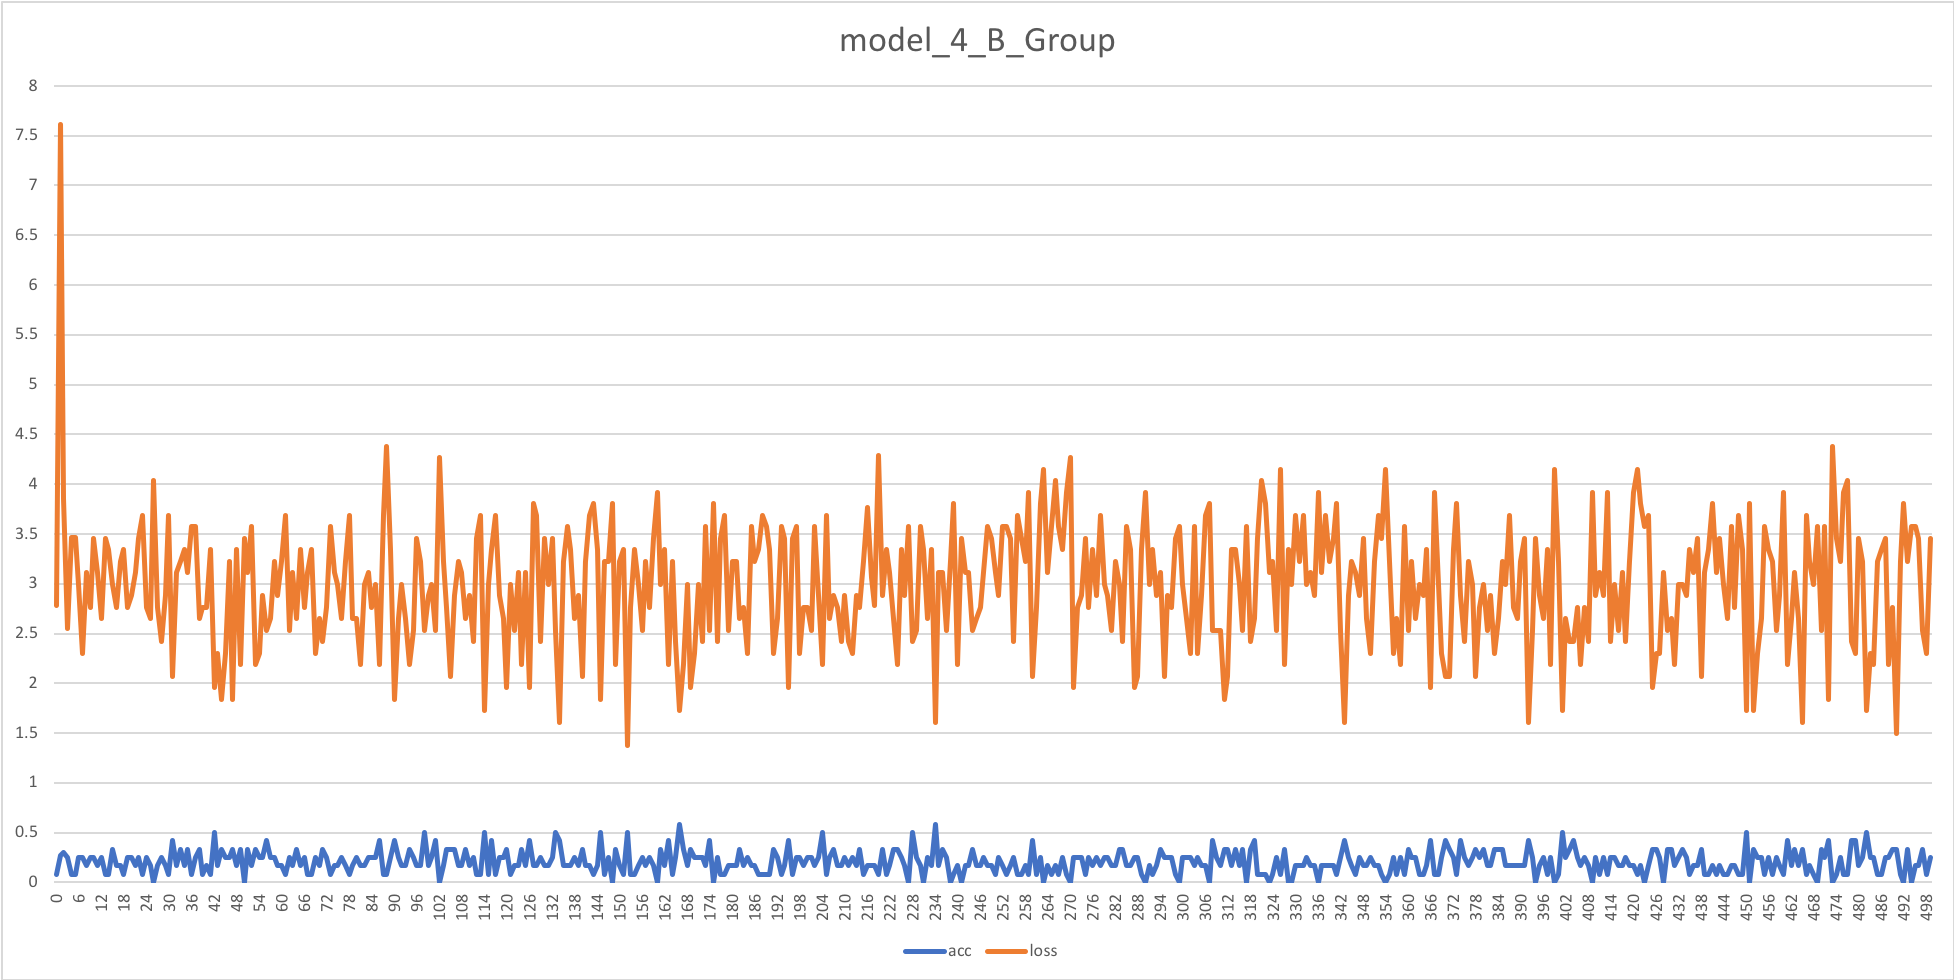
\includegraphics[width=0.5\textwidth]{charts/4B.png}
\caption{Training data of model 4 using augmented dataset}
\end{figure}

From the 4 pairs of images, Figure 7 and 8, Figure 9 and 10, Figure 11 and 12, Figure 13 and 14, showing the four models' performance when training with original dataset and augmented dataset, it can be seen that, when considering the scaling of y-axis, model 2, model 3 and model 4 displayed an improvement in accuracy when training with augmented dataset. The accuracy of model 2, model 3 and model 4 were normally below 0.5 when training with original dataset, while the accuracy of the same model was above 0.5 when training with augmented dataset. For model 1, training with augmented data does not have an accuracy lower than training with original data. Considering all above proof, we can come to conclusion that data augmentation can bring a certain degree of improvement on the accuracy of retinal disease diagnosis models. 

\begin{figure}[h]
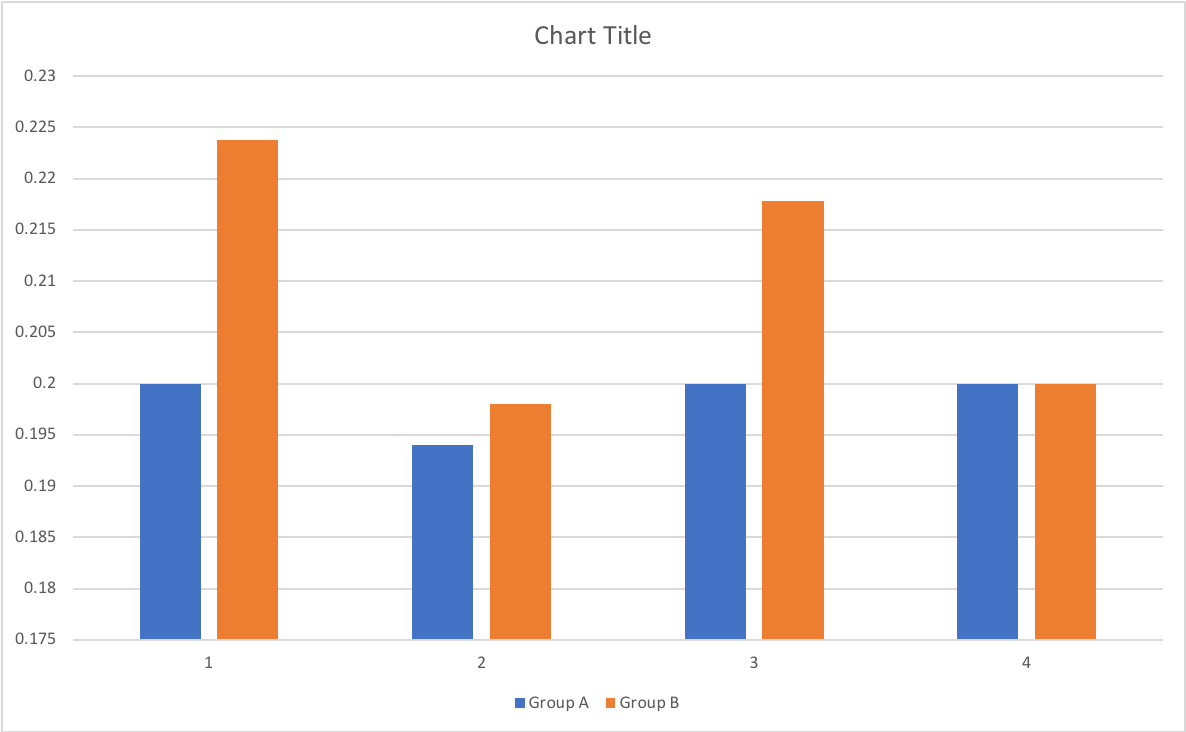
\includegraphics[width=0.5\textwidth]{charts/prediction result chart.png}
\caption{Prediction results: Group A uses the original dataset, Group B uses the augmented dataset.}
\end{figure}

On the other side, we write a python script to manually calculate the accuracy of our models' predictions. 505 images from the validation set, which have not been seen by the models when they are training, are used as prediction sample. The models provide five probability value corresponding to the five labels of severity of DR, and the label with largest value would be regarded as a prediction result of a single test case. The accuracy is calculated as total number of predictions that match the ground truth divided by total number of images tested. In Figure 15, we can observe that the Group B using the augmented dataset displays an improved prediction accuracy.
以表格的形式,分别列出几个模型(5个),在使用原始数据,和使用增强后的数据,得到的模型,其前后分类准确率。即使用增强后的数据,训练得到的模型,其准确率高于使用原始数据训练得到的模型。

从而证明,数据增强方法,能够提升基于深度学习方法的眼底疾病诊断准确率。

\subsection{实验分析}
We observe that the reason why data augmentation can improve retinal disease model's accuracy. It is because that by using data augmentation, more training examples can be provided, which solves the issue of unbalanced dataset. As mentioned above, the original dataset is extremely unbalanced, with 13423 images for degree 0, 1312 images for degree 1, 2755 for degree 2, 449 for degree 3 and 384 for degree 4. By using augmentation method, we can create an expanded and balanced retinal image dataset, with 13422 original images for degree 0, 13092 augmented images for degree 1, 13244 augmented images for degree 2, 13235 augmented images for degree 3, 13216 augmented images for degree 4. The augmentation method greatly increased the number of images for label 1, label 2, label 3 and label 4, as well as the overall size of the retinal image dataset. 
分析为什么数据增强方法,能够提升模型诊断眼底疾病的准确率。1、增加了训练样本数量。2、解决了各类别样本不均衡问题。

通过表格,罗列数据增强前后,每个类别图片数量,以及整个数据集图片总数量的对比。

% \section{总结}
\section{Conclusion}
进一步说明,使用数据增强方法,能够提升基于深度学习的眼底疾病诊断准确率。
From the experiment and analysis above, we can conclude that by using the method of data augmentation, we can improve the accuracy of retinal disease diagnosis powered by deep learning.

%% include bib file
\bibliographystyle{unsrt}
\bibliography{ijisa_sample}
   

\end{document}